\documentclass{article}


% if you need to pass options to natbib, use, e.g.:
%     \PassOptionsToPackage{numbers, compress}{natbib}
% before loading neurips_2023


% ready for submission
% \usepackage[preprint]{neurips_2024}
\usepackage{iclr2025_conference,times}
\iclrfinalcopy
%%%%% NEW MATH DEFINITIONS %%%%%

\usepackage{amsmath,amsfonts,bm}

% Mark sections of captions for referring to divisions of figures
\newcommand{\figleft}{{\em (Left)}}
\newcommand{\figcenter}{{\em (Center)}}
\newcommand{\figright}{{\em (Right)}}
\newcommand{\figtop}{{\em (Top)}}
\newcommand{\figbottom}{{\em (Bottom)}}
\newcommand{\captiona}{{\em (a)}}
\newcommand{\captionb}{{\em (b)}}
\newcommand{\captionc}{{\em (c)}}
\newcommand{\captiond}{{\em (d)}}

% Highlight a newly defined term
\newcommand{\newterm}[1]{{\bf #1}}


% Figure reference, lower-case.
\def\figref#1{figure~\ref{#1}}
% Figure reference, capital. For start of sentence
\def\Figref#1{Figure~\ref{#1}}
\def\twofigref#1#2{figures \ref{#1} and \ref{#2}}
\def\quadfigref#1#2#3#4{figures \ref{#1}, \ref{#2}, \ref{#3} and \ref{#4}}
% Section reference, lower-case.
\def\secref#1{section~\ref{#1}}
% Section reference, capital.
\def\Secref#1{Section~\ref{#1}}
% Reference to two sections.
\def\twosecrefs#1#2{sections \ref{#1} and \ref{#2}}
% Reference to three sections.
\def\secrefs#1#2#3{sections \ref{#1}, \ref{#2} and \ref{#3}}
% Reference to an equation, lower-case.
% \def\eqref#1{equation~\ref{#1}}
\def\eqref#1{(\ref{#1})}
% Reference to an equation, upper case
\def\Eqref#1{Equation~\ref{#1}}
% A raw reference to an equation---avoid using if possible
\def\plaineqref#1{\ref{#1}}
% Reference to a chapter, lower-case.
\def\chapref#1{chapter~\ref{#1}}
% Reference to an equation, upper case.
\def\Chapref#1{Chapter~\ref{#1}}
% Reference to a range of chapters
\def\rangechapref#1#2{chapters\ref{#1}--\ref{#2}}
% Reference to an algorithm, lower-case.
\def\algref#1{algorithm~\ref{#1}}
% Reference to an algorithm, upper case.
\def\Algref#1{Algorithm~\ref{#1}}
\def\twoalgref#1#2{algorithms \ref{#1} and \ref{#2}}
\def\Twoalgref#1#2{Algorithms \ref{#1} and \ref{#2}}
% Reference to a part, lower case
\def\partref#1{part~\ref{#1}}
% Reference to a part, upper case
\def\Partref#1{Part~\ref{#1}}
\def\twopartref#1#2{parts \ref{#1} and \ref{#2}}

\def\ceil#1{\lceil #1 \rceil}
\def\floor#1{\lfloor #1 \rfloor}
\def\1{\bm{1}}
\newcommand{\train}{\mathcal{D}}
\newcommand{\valid}{\mathcal{D_{\mathrm{valid}}}}
\newcommand{\test}{\mathcal{D_{\mathrm{test}}}}

\def\eps{{\epsilon}}


% Random variables
\def\reta{{\textnormal{$\eta$}}}
\def\ra{{\textnormal{a}}}
\def\rb{{\textnormal{b}}}
\def\rc{{\textnormal{c}}}
\def\rd{{\textnormal{d}}}
\def\re{{\textnormal{e}}}
\def\rf{{\textnormal{f}}}
\def\rg{{\textnormal{g}}}
\def\rh{{\textnormal{h}}}
\def\ri{{\textnormal{i}}}
\def\rj{{\textnormal{j}}}
\def\rk{{\textnormal{k}}}
\def\rl{{\textnormal{l}}}
% rm is already a command, just don't name any random variables m
\def\rn{{\textnormal{n}}}
\def\ro{{\textnormal{o}}}
\def\rp{{\textnormal{p}}}
\def\rq{{\textnormal{q}}}
\def\rr{{\textnormal{r}}}
\def\rs{{\textnormal{s}}}
\def\rt{{\textnormal{t}}}
\def\ru{{\textnormal{u}}}
\def\rv{{\textnormal{v}}}
\def\rw{{\textnormal{w}}}
\def\rx{{\textnormal{x}}}
\def\ry{{\textnormal{y}}}
\def\rz{{\textnormal{z}}}

% Random vectors
\def\rvepsilon{{\mathbf{\epsilon}}}
\def\rvtheta{{\mathbf{\theta}}}
\def\rva{{\mathbf{a}}}
\def\rvb{{\mathbf{b}}}
\def\rvc{{\mathbf{c}}}
\def\rvd{{\mathbf{d}}}
\def\rve{{\mathbf{e}}}
\def\rvf{{\mathbf{f}}}
\def\rvg{{\mathbf{g}}}
\def\rvh{{\mathbf{h}}}
\def\rvu{{\mathbf{i}}}
\def\rvj{{\mathbf{j}}}
\def\rvk{{\mathbf{k}}}
\def\rvl{{\mathbf{l}}}
\def\rvm{{\mathbf{m}}}
\def\rvn{{\mathbf{n}}}
\def\rvo{{\mathbf{o}}}
\def\rvp{{\mathbf{p}}}
\def\rvq{{\mathbf{q}}}
\def\rvr{{\mathbf{r}}}
\def\rvs{{\mathbf{s}}}
\def\rvt{{\mathbf{t}}}
\def\rvu{{\mathbf{u}}}
\def\rvv{{\mathbf{v}}}
\def\rvw{{\mathbf{w}}}
\def\rvx{{\mathbf{x}}}
\def\rvy{{\mathbf{y}}}
\def\rvz{{\mathbf{z}}}

% Elements of random vectors
\def\erva{{\textnormal{a}}}
\def\ervb{{\textnormal{b}}}
\def\ervc{{\textnormal{c}}}
\def\ervd{{\textnormal{d}}}
\def\erve{{\textnormal{e}}}
\def\ervf{{\textnormal{f}}}
\def\ervg{{\textnormal{g}}}
\def\ervh{{\textnormal{h}}}
\def\ervi{{\textnormal{i}}}
\def\ervj{{\textnormal{j}}}
\def\ervk{{\textnormal{k}}}
\def\ervl{{\textnormal{l}}}
\def\ervm{{\textnormal{m}}}
\def\ervn{{\textnormal{n}}}
\def\ervo{{\textnormal{o}}}
\def\ervp{{\textnormal{p}}}
\def\ervq{{\textnormal{q}}}
\def\ervr{{\textnormal{r}}}
\def\ervs{{\textnormal{s}}}
\def\ervt{{\textnormal{t}}}
\def\ervu{{\textnormal{u}}}
\def\ervv{{\textnormal{v}}}
\def\ervw{{\textnormal{w}}}
\def\ervx{{\textnormal{x}}}
\def\ervy{{\textnormal{y}}}
\def\ervz{{\textnormal{z}}}

% Random matrices
\def\rmA{{\mathbf{A}}}
\def\rmB{{\mathbf{B}}}
\def\rmC{{\mathbf{C}}}
\def\rmD{{\mathbf{D}}}
\def\rmE{{\mathbf{E}}}
\def\rmF{{\mathbf{F}}}
\def\rmG{{\mathbf{G}}}
\def\rmH{{\mathbf{H}}}
\def\rmI{{\mathbf{I}}}
\def\rmJ{{\mathbf{J}}}
\def\rmK{{\mathbf{K}}}
\def\rmL{{\mathbf{L}}}
\def\rmM{{\mathbf{M}}}
\def\rmN{{\mathbf{N}}}
\def\rmO{{\mathbf{O}}}
\def\rmP{{\mathbf{P}}}
\def\rmQ{{\mathbf{Q}}}
\def\rmR{{\mathbf{R}}}
\def\rmS{{\mathbf{S}}}
\def\rmT{{\mathbf{T}}}
\def\rmU{{\mathbf{U}}}
\def\rmV{{\mathbf{V}}}
\def\rmW{{\mathbf{W}}}
\def\rmX{{\mathbf{X}}}
\def\rmY{{\mathbf{Y}}}
\def\rmZ{{\mathbf{Z}}}

% Elements of random matrices
\def\ermA{{\textnormal{A}}}
\def\ermB{{\textnormal{B}}}
\def\ermC{{\textnormal{C}}}
\def\ermD{{\textnormal{D}}}
\def\ermE{{\textnormal{E}}}
\def\ermF{{\textnormal{F}}}
\def\ermG{{\textnormal{G}}}
\def\ermH{{\textnormal{H}}}
\def\ermI{{\textnormal{I}}}
\def\ermJ{{\textnormal{J}}}
\def\ermK{{\textnormal{K}}}
\def\ermL{{\textnormal{L}}}
\def\ermM{{\textnormal{M}}}
\def\ermN{{\textnormal{N}}}
\def\ermO{{\textnormal{O}}}
\def\ermP{{\textnormal{P}}}
\def\ermQ{{\textnormal{Q}}}
\def\ermR{{\textnormal{R}}}
\def\ermS{{\textnormal{S}}}
\def\ermT{{\textnormal{T}}}
\def\ermU{{\textnormal{U}}}
\def\ermV{{\textnormal{V}}}
\def\ermW{{\textnormal{W}}}
\def\ermX{{\textnormal{X}}}
\def\ermY{{\textnormal{Y}}}
\def\ermZ{{\textnormal{Z}}}

% Vectors
\def\vzero{{\bm{0}}}
\def\vone{{\bm{1}}}
\def\vmu{{\bm{\mu}}}
\def\vtheta{{\bm{\theta}}}
\def\va{{\bm{a}}}
\def\vb{{\bm{b}}}
\def\vc{{\bm{c}}}
\def\vd{{\bm{d}}}
\def\ve{{\bm{e}}}
\def\vf{{\bm{f}}}
\def\vg{{\bm{g}}}
\def\vh{{\bm{h}}}
\def\vi{{\bm{i}}}
\def\vj{{\bm{j}}}
\def\vk{{\bm{k}}}
\def\vl{{\bm{l}}}
\def\vm{{\bm{m}}}
\def\vn{{\bm{n}}}
\def\vo{{\bm{o}}}
\def\vp{{\bm{p}}}
\def\vq{{\bm{q}}}
\def\vr{{\bm{r}}}
\def\vs{{\bm{s}}}
\def\vt{{\bm{t}}}
\def\vu{{\bm{u}}}
\def\vv{{\bm{v}}}
\def\vw{{\bm{w}}}
\def\vx{{\bm{x}}}
\def\vy{{\bm{y}}}
\def\vz{{\bm{z}}}

% Elements of vectors
\def\evalpha{{\alpha}}
\def\evbeta{{\beta}}
\def\evepsilon{{\epsilon}}
\def\evlambda{{\lambda}}
\def\evomega{{\omega}}
\def\evmu{{\mu}}
\def\evpsi{{\psi}}
\def\evsigma{{\sigma}}
\def\evtheta{{\theta}}
\def\eva{{a}}
\def\evb{{b}}
\def\evc{{c}}
\def\evd{{d}}
\def\eve{{e}}
\def\evf{{f}}
\def\evg{{g}}
\def\evh{{h}}
\def\evi{{i}}
\def\evj{{j}}
\def\evk{{k}}
\def\evl{{l}}
\def\evm{{m}}
\def\evn{{n}}
\def\evo{{o}}
\def\evp{{p}}
\def\evq{{q}}
\def\evr{{r}}
\def\evs{{s}}
\def\evt{{t}}
\def\evu{{u}}
\def\evv{{v}}
\def\evw{{w}}
\def\evx{{x}}
\def\evy{{y}}
\def\evz{{z}}

% Matrix
\def\mA{{\bm{A}}}
\def\mB{{\bm{B}}}
\def\mC{{\bm{C}}}
\def\mD{{\bm{D}}}
\def\mE{{\bm{E}}}
\def\mF{{\bm{F}}}
\def\mG{{\bm{G}}}
\def\mH{{\bm{H}}}
\def\mI{{\bm{I}}}
\def\mJ{{\bm{J}}}
\def\mK{{\bm{K}}}
\def\mL{{\bm{L}}}
\def\mM{{\bm{M}}}
\def\mN{{\bm{N}}}
\def\mO{{\bm{O}}}
\def\mP{{\bm{P}}}
\def\mQ{{\bm{Q}}}
\def\mR{{\bm{R}}}
\def\mS{{\bm{S}}}
\def\mT{{\bm{T}}}
\def\mU{{\bm{U}}}
\def\mV{{\bm{V}}}
\def\mW{{\bm{W}}}
\def\mX{{\bm{X}}}
\def\mY{{\bm{Y}}}
\def\mZ{{\bm{Z}}}
\def\mBeta{{\bm{\beta}}}
\def\mPhi{{\bm{\Phi}}}
\def\mLambda{{\bm{\Lambda}}}
\def\mSigma{{\bm{\Sigma}}}

% Tensor
\DeclareMathAlphabet{\mathsfit}{\encodingdefault}{\sfdefault}{m}{sl}
\SetMathAlphabet{\mathsfit}{bold}{\encodingdefault}{\sfdefault}{bx}{n}
\newcommand{\tens}[1]{\bm{\mathsfit{#1}}}
\def\tA{{\tens{A}}}
\def\tB{{\tens{B}}}
\def\tC{{\tens{C}}}
\def\tD{{\tens{D}}}
\def\tE{{\tens{E}}}
\def\tF{{\tens{F}}}
\def\tG{{\tens{G}}}
\def\tH{{\tens{H}}}
\def\tI{{\tens{I}}}
\def\tJ{{\tens{J}}}
\def\tK{{\tens{K}}}
\def\tL{{\tens{L}}}
\def\tM{{\tens{M}}}
\def\tN{{\tens{N}}}
\def\tO{{\tens{O}}}
\def\tP{{\tens{P}}}
\def\tQ{{\tens{Q}}}
\def\tR{{\tens{R}}}
\def\tS{{\tens{S}}}
\def\tT{{\tens{T}}}
\def\tU{{\tens{U}}}
\def\tV{{\tens{V}}}
\def\tW{{\tens{W}}}
\def\tX{{\tens{X}}}
\def\tY{{\tens{Y}}}
\def\tZ{{\tens{Z}}}


% Graph
\def\gA{{\mathcal{A}}}
\def\gB{{\mathcal{B}}}
\def\gC{{\mathcal{C}}}
\def\gD{{\mathcal{D}}}
\def\gE{{\mathcal{E}}}
\def\gF{{\mathcal{F}}}
\def\gG{{\mathcal{G}}}
\def\gH{{\mathcal{H}}}
\def\gI{{\mathcal{I}}}
\def\gJ{{\mathcal{J}}}
\def\gK{{\mathcal{K}}}
\def\gL{{\mathcal{L}}}
\def\gM{{\mathcal{M}}}
\def\gN{{\mathcal{N}}}
\def\gO{{\mathcal{O}}}
\def\gP{{\mathcal{P}}}
\def\gQ{{\mathcal{Q}}}
\def\gR{{\mathcal{R}}}
\def\gS{{\mathcal{S}}}
\def\gT{{\mathcal{T}}}
\def\gU{{\mathcal{U}}}
\def\gV{{\mathcal{V}}}
\def\gW{{\mathcal{W}}}
\def\gX{{\mathcal{X}}}
\def\gY{{\mathcal{Y}}}
\def\gZ{{\mathcal{Z}}}

% Sets
\def\sA{{\mathbb{A}}}
\def\sB{{\mathbb{B}}}
\def\sC{{\mathbb{C}}}
\def\sD{{\mathbb{D}}}
% Don't use a set called E, because this would be the same as our symbol
% for expectation.
\def\sF{{\mathbb{F}}}
\def\sG{{\mathbb{G}}}
\def\sH{{\mathbb{H}}}
\def\sI{{\mathbb{I}}}
\def\sJ{{\mathbb{J}}}
\def\sK{{\mathbb{K}}}
\def\sL{{\mathbb{L}}}
\def\sM{{\mathbb{M}}}
\def\sN{{\mathbb{N}}}
\def\sO{{\mathbb{O}}}
\def\sP{{\mathbb{P}}}
\def\sQ{{\mathbb{Q}}}
\def\sR{{\mathbb{R}}}
\def\sS{{\mathbb{S}}}
\def\sT{{\mathbb{T}}}
\def\sU{{\mathbb{U}}}
\def\sV{{\mathbb{V}}}
\def\sW{{\mathbb{W}}}
\def\sX{{\mathbb{X}}}
\def\sY{{\mathbb{Y}}}
\def\sZ{{\mathbb{Z}}}

% Entries of a matrix
\def\emLambda{{\Lambda}}
\def\emA{{A}}
\def\emB{{B}}
\def\emC{{C}}
\def\emD{{D}}
\def\emE{{E}}
\def\emF{{F}}
\def\emG{{G}}
\def\emH{{H}}
\def\emI{{I}}
\def\emJ{{J}}
\def\emK{{K}}
\def\emL{{L}}
\def\emM{{M}}
\def\emN{{N}}
\def\emO{{O}}
\def\emP{{P}}
\def\emQ{{Q}}
\def\emR{{R}}
\def\emS{{S}}
\def\emT{{T}}
\def\emU{{U}}
\def\emV{{V}}
\def\emW{{W}}
\def\emX{{X}}
\def\emY{{Y}}
\def\emZ{{Z}}
\def\emSigma{{\Sigma}}

% entries of a tensor
% Same font as tensor, without \bm wrapper
\newcommand{\etens}[1]{\mathsfit{#1}}
\def\etLambda{{\etens{\Lambda}}}
\def\etA{{\etens{A}}}
\def\etB{{\etens{B}}}
\def\etC{{\etens{C}}}
\def\etD{{\etens{D}}}
\def\etE{{\etens{E}}}
\def\etF{{\etens{F}}}
\def\etG{{\etens{G}}}
\def\etH{{\etens{H}}}
\def\etI{{\etens{I}}}
\def\etJ{{\etens{J}}}
\def\etK{{\etens{K}}}
\def\etL{{\etens{L}}}
\def\etM{{\etens{M}}}
\def\etN{{\etens{N}}}
\def\etO{{\etens{O}}}
\def\etP{{\etens{P}}}
\def\etQ{{\etens{Q}}}
\def\etR{{\etens{R}}}
\def\etS{{\etens{S}}}
\def\etT{{\etens{T}}}
\def\etU{{\etens{U}}}
\def\etV{{\etens{V}}}
\def\etW{{\etens{W}}}
\def\etX{{\etens{X}}}
\def\etY{{\etens{Y}}}
\def\etZ{{\etens{Z}}}

% The true underlying data generating distribution
\newcommand{\pdata}{p_{\rm{data}}}
% The empirical distribution defined by the training set
\newcommand{\ptrain}{\hat{p}_{\rm{data}}}
\newcommand{\Ptrain}{\hat{P}_{\rm{data}}}
% The model distribution
\newcommand{\pmodel}{p_{\rm{model}}}
\newcommand{\Pmodel}{P_{\rm{model}}}
\newcommand{\ptildemodel}{\tilde{p}_{\rm{model}}}
% Stochastic autoencoder distributions
\newcommand{\pencode}{p_{\rm{encoder}}}
\newcommand{\pdecode}{p_{\rm{decoder}}}
\newcommand{\precons}{p_{\rm{reconstruct}}}

\newcommand{\laplace}{\mathrm{Laplace}} % Laplace distribution

\newcommand{\E}{\mathbb{E}}
\newcommand{\Ls}{\mathcal{L}}
\newcommand{\R}{\mathbb{R}}
\newcommand{\emp}{\tilde{p}}
\newcommand{\lr}{\alpha}
\newcommand{\reg}{\lambda}
\newcommand{\rect}{\mathrm{rectifier}}
\newcommand{\softmax}{\mathrm{softmax}}
\newcommand{\sigmoid}{\sigma}
\newcommand{\softplus}{\zeta}
\newcommand{\KL}{D_{\mathrm{KL}}}
\newcommand{\Var}{\mathrm{Var}}
\newcommand{\standarderror}{\mathrm{SE}}
\newcommand{\Cov}{\mathrm{Cov}}
% Wolfram Mathworld says $L^2$ is for function spaces and $\ell^2$ is for vectors
% But then they seem to use $L^2$ for vectors throughout the site, and so does
% wikipedia.
\newcommand{\normlzero}{L^0}
\newcommand{\normlone}{L^1}
\newcommand{\normltwo}{L^2}
\newcommand{\normlp}{L^p}
\newcommand{\normmax}{L^\infty}

\newcommand{\parents}{Pa} % See usage in notation.tex. Chosen to match Daphne's book.

\DeclareMathOperator*{\argmax}{arg\,max}
\DeclareMathOperator*{\argmin}{arg\,min}

\DeclareMathOperator{\sign}{sign}
\DeclareMathOperator{\Tr}{Tr}
\let\ab\allowbreak

% to compile a preprint version, e.g., for submission to arXiv, add add the
% [preprint] option:
%     \usepackage[preprint]{neurips_2023}


% to compile a camera-ready version, add the [final] option, e.g.:
%     \usepackage[final]{neurips_2023}


% to avoid loading the natbib package, add option nonatbib:
%    \usepackage[nonatbib]{neurips_2023}

\usepackage[utf8]{inputenc} % allow utf-8 input
\usepackage[T1]{fontenc}    % use 8-bit T1 fonts
\usepackage{hyperref}       % hyperlinks
\usepackage{url}            % simple URL typesetting
\usepackage{booktabs}       % professional-quality tables
\usepackage{amsfonts}       % blackboard math symbols
\usepackage{nicefrac}       % compact symbols for 1/2, etc.
\usepackage{microtype}      % microtypography
\usepackage{xcolor}         % colors
\usepackage{graphicx}
\usepackage{multirow}
\usepackage{amsmath}        % aligned equations
\usepackage{bbm}
\usepackage{mathrsfs}
% \usepackage{emoji}
\usepackage{makecell}
\usepackage{subcaption} 
\usepackage{marvosym}
\usepackage{amsmath}
\usepackage{amssymb}

\newcommand{\tabincell}[2]{\begin{tabular}{@{}#1@{}}#2\end{tabular}} 

\usepackage{newfloat}
\usepackage{tcolorbox}
\usepackage{lipsum}
\usepackage{listings}
\usepackage{courier}
\usepackage{wrapfig}



\def\eg{\emph{e.g.}} \def\Eg{\emph{E.g.}}
\def\ie{\emph{i.e}} \def\Ie{\emph{I.e.}}
\def\cf{\emph{c.f.}} \def\Cf{\emph{C.f.}}
\def\etc{\emph{etc}} \def\vs{\emph{vs.}}
\def\wrt{w.r.t.} \def\dof{d.o.f.}
\def\etal{\emph{et al.}}


\title{UnrealZoo: Enriching Photo-realistic Virtual Worlds for Embodied AI}


\author{
Fangwei Zhong\textsuperscript{*$\sharp$$\dagger$}
Kui Wu\textsuperscript{*$\S$}
Churan Wang\textsuperscript{$\ddag$}
Hao Chen\textsuperscript{$\between$}
Hai Ci\textsuperscript{$\lozenge$}
Zhoujun Li\textsuperscript{$\S$}
Yizhou Wang\textsuperscript{$\ddag$}\\
\textsuperscript{$\sharp$} Beijing Normal University  
\textsuperscript{$\S$} Beihang University  
\textsuperscript{$\ddag$} Peking University 
\\
\textsuperscript{$\dagger$} BIGAI 
\textsuperscript{$\between$} City University of Macau  
\textsuperscript{$\lozenge$} National University of Singapore\\
\textsuperscript{*} indicates equal contribution, 
\Letter correspondence to: \texttt{fangweizhong@bnu.edu.cn} \\
}


\begin{document}


\maketitle

\vspace{-0.3cm}
\begin{abstract}

We introduce UnrealZoo~\footnote{Project page: \url{http://unrealzoo.site/}}, a rich collection of photo-realistic 3D virtual worlds built on Unreal Engine, designed to reflect the complexity and variability of the open worlds. Additionally, we offer a variety of playable entities for embodied AI agents. Based on UnrealCV, we provide a suite of easy-to-use Python APIs and tools for various potential applications, such as data collection, environment augmentation, distributed training, and benchmarking.
We optimize the rendering and communication efficiency of UnrealCV to support advanced applications, such as multi-agent interaction.
Our experiments benchmark agents in various complex scenes, focusing on visual navigation and tracking, which are fundamental capabilities for embodied visual intelligence.
The results yield valuable insights into the advantages of diverse training environments for reinforcement learning (RL) agents and the challenges faced by current embodied vision agents, including those based on RL and large vision-language models (VLMs), in open worlds. These challenges involve latency in closed-loop control in dynamic scenes and reasoning about 3D spatial structures in unstructured terrain.
\vspace{-0.3cm}
\end{abstract} 

\begin{figure*}[h]
    \centering
    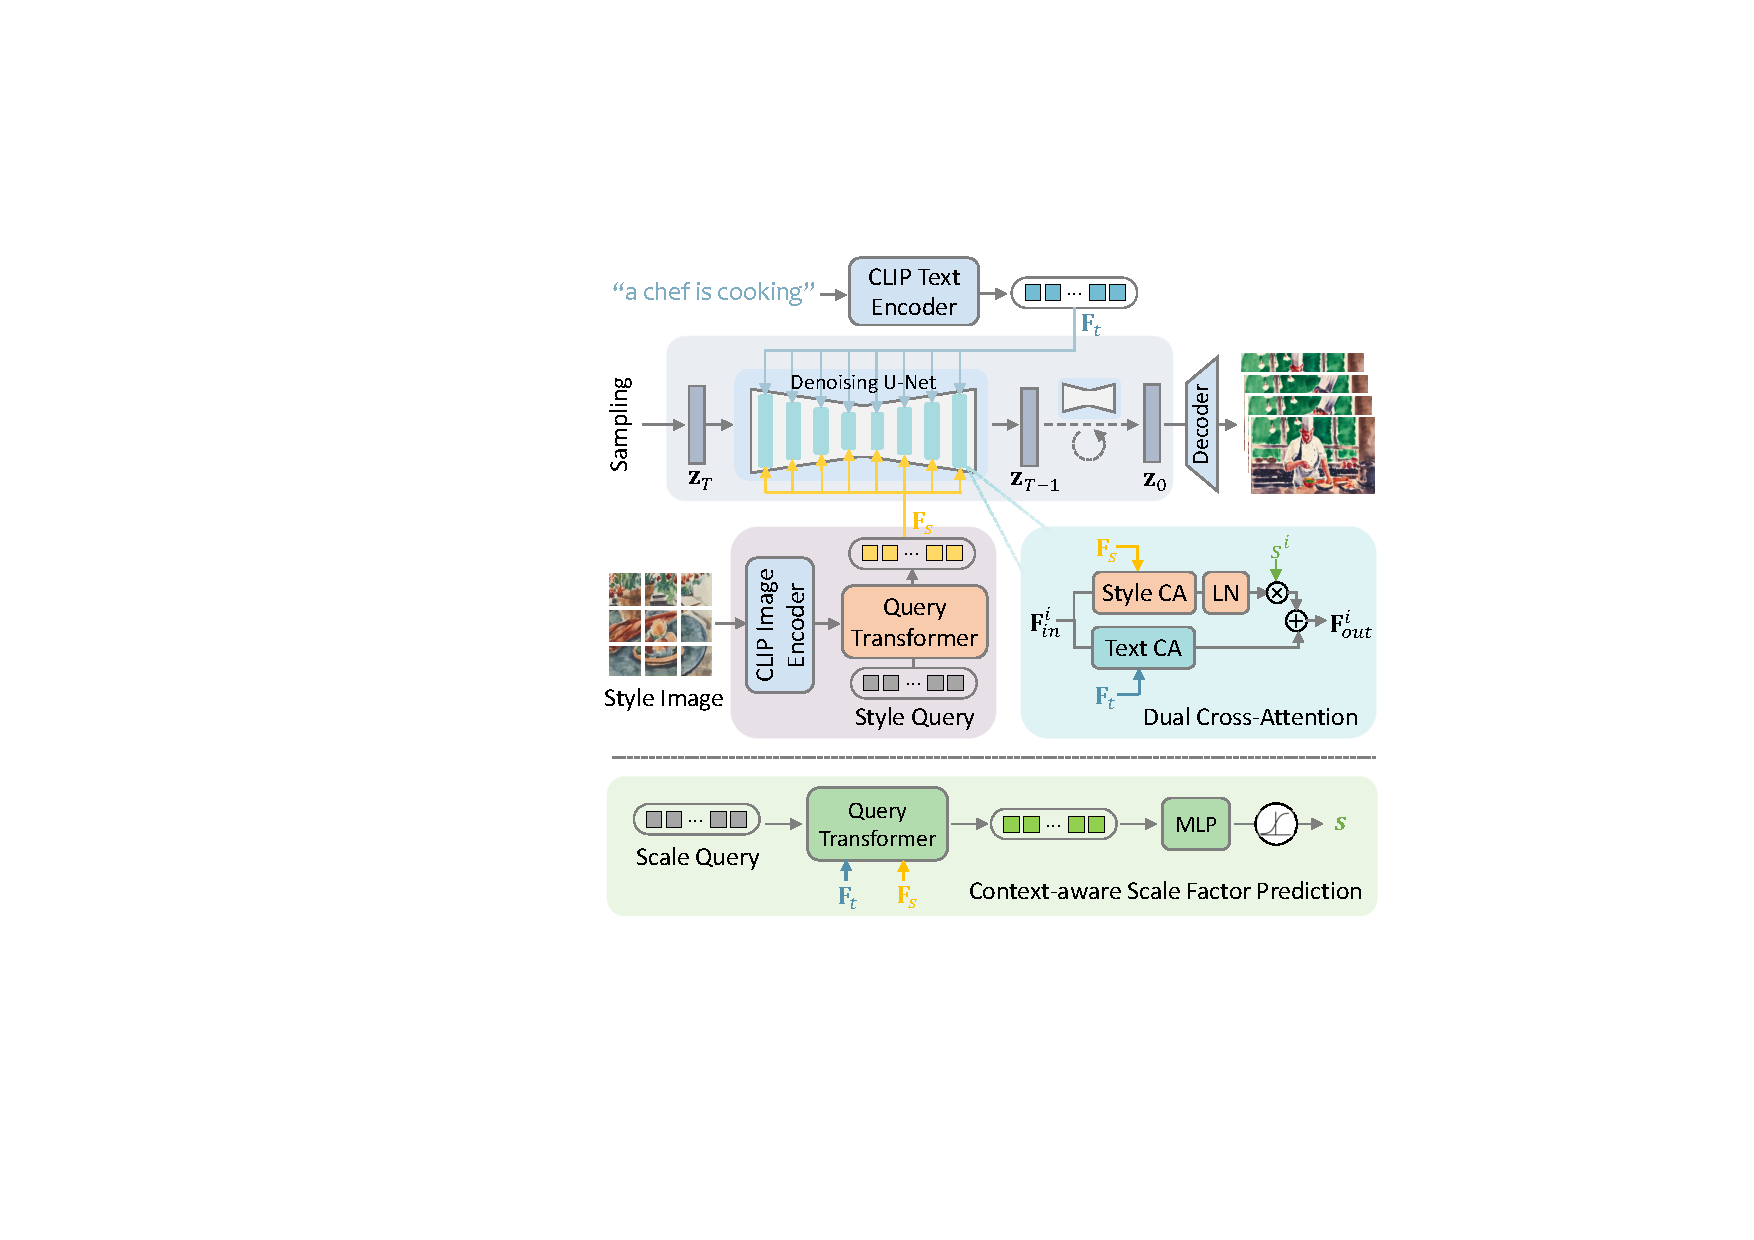
\includegraphics[width=0.99\textwidth]{image/overview2.pdf}
    \caption{
    UnrealZoo enriches photo-realistic virtual worlds by combining diverse scenes and playable entities. It enables training generalizable embodied AI agents for tasks such as navigation, active tracking, and social interactions. Additionally, UnrealZoo facilitates the benchmarking of agents in realistic virtual worlds, helping to identify challenges in open-world deployments.
    }
    \label{fig:overview}
\end{figure*}

\section{Introduction}


Currently, embodied artificial intelligence (Embodied AI) agents are often \textit{homebodies}, primarily confined to controlled indoor environments and rarely venturing outside to explore the diversity of the open world.  
While several simulators~\citep{kolve2017ai2, CARLA, puig2018virtualhome, li2023behavior,   puig2023habitat} have advanced the field, they often focus on specific scenarios, such as daily activities in homes or autonomous driving on urban roads.
This narrow focus hinders AI agents' adaptability and generalization in diverse open worlds, e.g., industrial areas, public spaces, and natural landscapes, required by a wide range of real-world applications.

To bridge this gap, there is an increasing demand for simulators that feature a diverse range of open worlds. 
\emph{First}, the diversity of the 3D scenes and bodies of agents is crucial to develop spatial intelligence~\citep{davison2018futuremapping}, enabling agents to actively perceive, reason, plan, and act when handling numerous tasks in complex 3D worlds with varying dynamics and styles.
\emph{Second}, the complexity of multi-agent interactions is essential for developing social intelligence~\citep{duenez2023social}, such as the theory of mind~\citep{jin-etal-2024-mmtom}, negotiation~\citep{guan2024richelieu}, cooperation~\citep{wang2022tomc}, and competition~\citep{zhong2021distractor}, encouraging agents to behave more like humans.
\emph{Third}, virtual worlds that mimic the challenges in open-world scenarios can evaluate agents efficiently and effectively, identifying limitations and preventing hardware losses from real-world deployment failures~\citep{kadian2020sim2real}.
\emph{Ultimately}, these features will inspire researchers to explore new challenges previously overlooked in other simulators~\citep{duan2022survey}, facilitating seamless integration into real-world applications.


In this work, we introduce UnrealZoo, a comprehensive collection of photo-realistic virtual worlds, based on Unreal Engine~\footnote{www.unrealengine.com} and UnrealCV~\citep{qiu2017unrealcv}. UnrealZoo features a diverse range of complex open worlds and playable entities to advance research in embodied AI and related domains. 
This high-quality set includes 100 realistic scenes at varying scales, such as houses, supermarkets, train stations, industrial factories, urban cities, villages, temples, and natural landscapes.
Each environment is expertly designed by artists to mimic realistic lighting, textures, and dynamics, closely resembling real-world experiences.
Our collection also includes diverse playable entities, including humans, animals, robots, drones, motorbikes, and cars. This diversity enables researchers to investigate the generalization of agents across different embodiments or build complex 3D social worlds with numerous heterogeneous agents.
To enhance usability, we further optimize UnrealCV and offer a suite of easy-to-use Python APIs and tools (UnrealCV+), including environment augmentation, demonstration collection, and distributed training/testing. These tools allow for customization and extension of the environments to meet various needs in future applications, ensuring UnrealZoo remains adaptable as the embodied AI agents evolve.

We conduct experiments to demonstrate the applicability of UnrealZoo for embodied AI. First, we benchmark frames per second (FPS) across various commands, highlighting the significant improvement in image rendering and multi-agent interactions with the UnrealCV+ API. We use embodied visual navigation~\citep{thor2017} and tracking~\citep{luo2018end, zhong2021distractor} as two example tasks to benchmark embodied vision agents in complex dynamic environments with moving objects and unstructured maps. We also introduce a set of simple yet effective baseline methods for developing embodied vision agents, including distributed online reinforcement learning algorithms~\citep{mnih2016asynchronous}, offline reinforcement learning algorithms~\citep{kumar2020conservative}, and a reasoning framework for large vision-language models (VLMs). Our evaluations across different settings emphasize the importance of diverse training environments for enhancing agent generalization and robustness, the necessity of low latency in closed-loop control to handle dynamic factors, and the potential of reinforcement learning for training agents to navigate complex scenes.

Our contributions can be summarized in the following:
1) We build UnrealZoo, a collection of 100 high-quality photo-realistic scenes and a set of playable entities with diverse features, covering the most challenging to embodied AI agents in open worlds.
2) We optimize the communication efficiency of UnrealCV APIs and provide easy-to-use Gym interfaces with a toolkit for diverse requirements.
3) We conduct experiments to demonstrate the usability of UnrealZoo, showing the importance of the diversity of the environments to the embodied agents, and analyzing the limitations of the current RL-based and VLM-based agents in the open worlds.



\section{Related Works}

\textbf{Realistic Simulators for Embodied AI.}
Realistic simulators are extensively utilized in embodied artificial intelligence due to their appealing benefits, including high-quality rendering, cost-effective ground truth generation, low-cost interaction, and environmental controllability. They are crucial for training and testing AI agents to handle increasingly complex tasks. Notable realistic 3D simulators have been created for specific applications, such as indoor navigation~\citep{kolve2017ai2, puig2018virtualhome, xia2018gibson, house3D}, robot manipulation~\citep{yu2020meta, ehsani2021manipulathor, chen2023bi}, and autonomous driving~\citep{virtual_kitti, airsim,  CARLA}.
Recent advances in computer graphics have spurred interest in developing general-purpose virtual worlds with photo-realistic rendering, allowing agents to collect high-fidelity data and learn skills applicable across various tasks and scenes. ThreeDWorlds (TDW)~\citep{gan2020threedworld} and LEGENT~\citep{cheng2024legent} are notable simulators that offer photo-realistic, multi-modal platforms, based on Unity, for interactive physical simulation. However, their built-in scenes and playable entities are somewhat limited. Additionally, the performance of the simulator decreases significantly in large outdoor environments, a typical weakness of Unity. V-IRL~\citep{yang2024v} is a recent approach that leverages Google Maps' API to simulate agents with real-world street view images, significantly reducing the gap between virtual and real-world settings. However, since V-IRL is inherently composed of static images, it lacks the capability to simulate the dynamics of the physical worlds for agent-object interactions.
Recently, the community has also begun to explore dynamic environments with social interactions and unexpected events. However, existing solutions like Habitat 3.0~\citep{puig2023habitat} focus on a limited number of agent interactions in indoor scenes, while HAZARD~\citep{zhou2024hazard} addresses only single-agent simulations in dynamic scenarios like fires, floods, and winds. In contrast, UnrealZoo offers a comprehensive collection of scenes that feature various scenes at different scales, situations, eras, and cultural backgrounds with diverse playable entities for embodied AI. With advancements in Unreal Engine and optimized UnrealCV, our environment achieves real-time performance in large-scale scenes with multiple agents (around 10) and photo-realistic rendering.
A comprehensive comparison across the related photo-realistic simulators is shown in Table~\ref{tab:env_comparision}.




\begin{table}[t]
\centering
    \caption{The comparison with related photo-realistic virtual worlds for embodied AI. \textbf{Unstr. Terr.} indicates the presence of unstructured terrain. \textbf{Nav. Sys.} specifies whether the agent in the environment includes an autonomous navigation system. In Appendix~\ref{app:env}, we compare the visual realism across different engines in Figure~\ref{fig: visual_realism} and list the descriptions of the symbols in Table~\ref{tab:symbol}.}
\label{tab:env_comparision}
\begin{tabular}{c}
\begin{minipage}{1\textwidth}
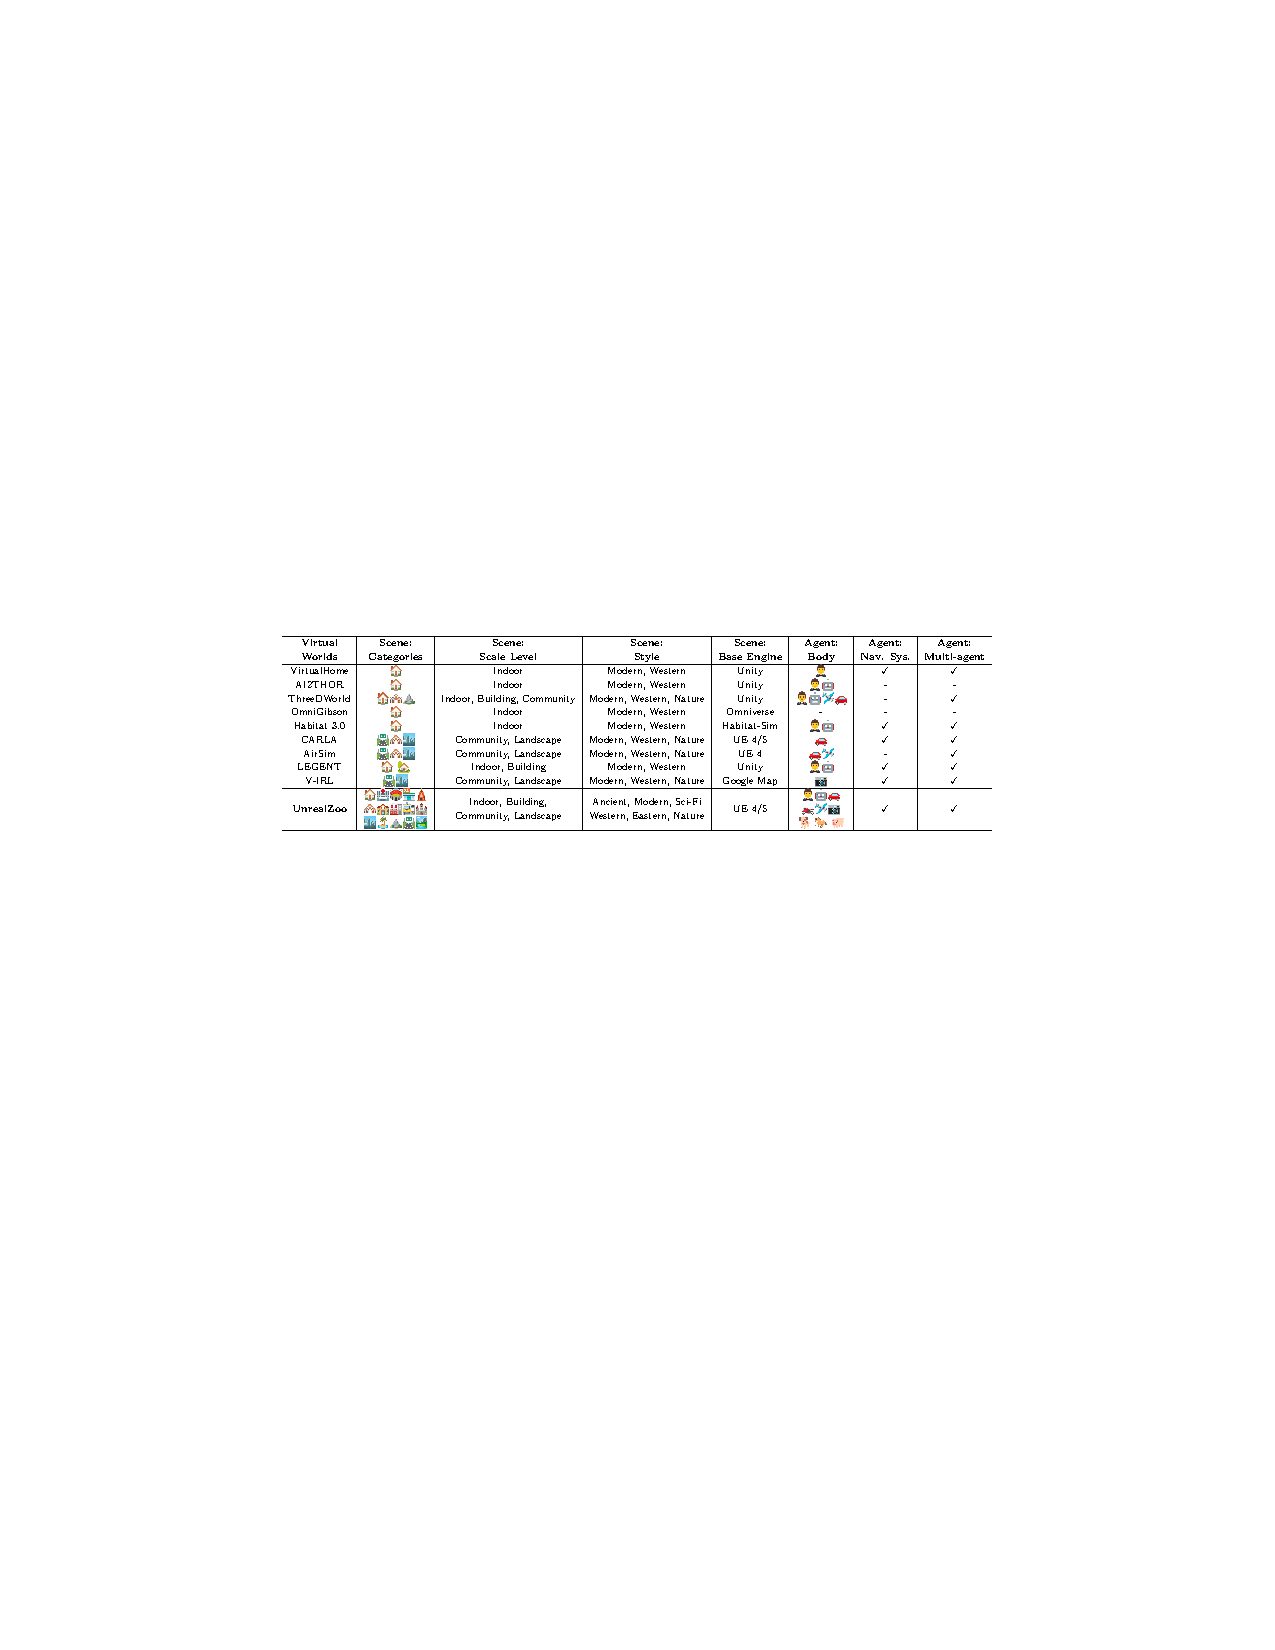
\includegraphics[width=\linewidth]{image/Compare_sim.pdf}
\end{minipage} 
\end{tabular}
\vspace{-0.5cm}
\end{table}


\renewcommand{\arraystretch}{1.1}

\textbf{Embodied Vision Agents.}
Embodied vision agents, which perceive and interact with their environments through vision, are a key focus in artificial intelligence research. These agents perform tasks like navigation~\citep{thor2017, gupta2017cognitive, yokoyama2024vlfm, long2024instructnav}, active object tracking~\citep{luo2018end, zhong2018advat, zhong2021distractor, zhong2023rspt, zhong2024empowering}, and other interactive tasks~\citep{chaplot2020learning, weihs2021visual, ci2023proactive, wang2023rearrange}, mimicking human behavior. Their development involves various methods, including state representation learning~\citep{yadav2023offline, yuan2022pre, gadre2022continuous, yang2023track}, reinforcement learning (RL)~\citep{schulman2017proximal, xu2023drm, ma2023revisiting}, and large vision-language models (VLMs)~\citep{zhang2024navid, zhou2024navgpt}.
Despite significant progress, challenges remain. RL methods often require extensive trial-and-error interactions and computational resources for training, and they usually struggle to generalize to new environments. Conversely, VLM-based methods excel at interpreting language instructions and images but may lack the fine-grained control and adaptability necessary for real-time interactions. The computational demands and time needed for inference with such large models are critical, especially in dynamic scenes.
Moreover, previous simulators mainly focus on indoor rooms or urban roads, which mask the potential challenges to the embodied agents when deploying in open worlds, e.g., unstructured terrain, dynamic changing factors, inference costs of the perception-control loop, and social interactions with other agents. Therefore, it is required to benchmark agents in large-scale, photo-realistic open worlds, taking into account various real-world challenges in the virtual worlds. In this work, we collect a subset of environments from UnrealZoo and benchmark embodied visual navigation and tracking agents, to emphasize the weakness of the existing RL-based and VLM-based methods.

\vspace{-0.3cm}
\section{UnrealZoo}
\vspace{-0.2cm}
UnrealZoo is a collection of photo-realistic, interactive open-world environments with diverse embodied characters, built on Unreal Engine and UnrealCV~\citep{qiu2017unrealcv}.
The environments are sourced from the \emph{Unreal Engine Marketplace}~\footnote{https://www.unrealengine.com/marketplace}, which shares high-quality content from artists, and were accumulated over two years at a cost exceeding $10,000$.
UnrealZoo features a diverse array of scenes with varying sizes and styles. Among them, the largest scene, i.e., Medieval Nature Environment, covers more than $16 km^2$ areas. 
The environments also include a wide range of embodiment, such as human avatars, vehicles, drones, animals, and virtual cameras, all of which can interact with the environment and equipped with ego-centric sensing systems.
We offer easy-to-use Python APIs based on UnrealCV to facilitate interaction between Python programs and the game engine. 
Note that UnrealCV is optimized for rendering and communication, particularly in large-scale and multi-agent scenarios, namely UnrealCV+.
Additionally, we provide OpenAI Gym interfaces to standardize agent-environment interactions.
The gym-like interface also contains a set of toolkits, e.g., environment augmentation, population control, time dilation, and JSON-style task configurations to help the user customize the environments for various tasks with minimal effort.
% The \href{http://unrealzoo.site/}{project website} includes the details of the collected contents, and documents about tutorials, Python APIs, and the gym interface.

\subsection{Scene Collection}

UnrealCV Zoo contains 100 scenes based on Unreal Engine 4 and 5. 
We select the scene based on the public reviews in the marketplace and the difference between the collected scenes, aiming at covering a wide range of styles from ancient to fictional, ensuring diversity. We provide an overview of the environments in the 
\href{https://unrealzoo.notion.site/scene-gallery}{scene gallery}.

\begin{figure}[t]
    \centering
    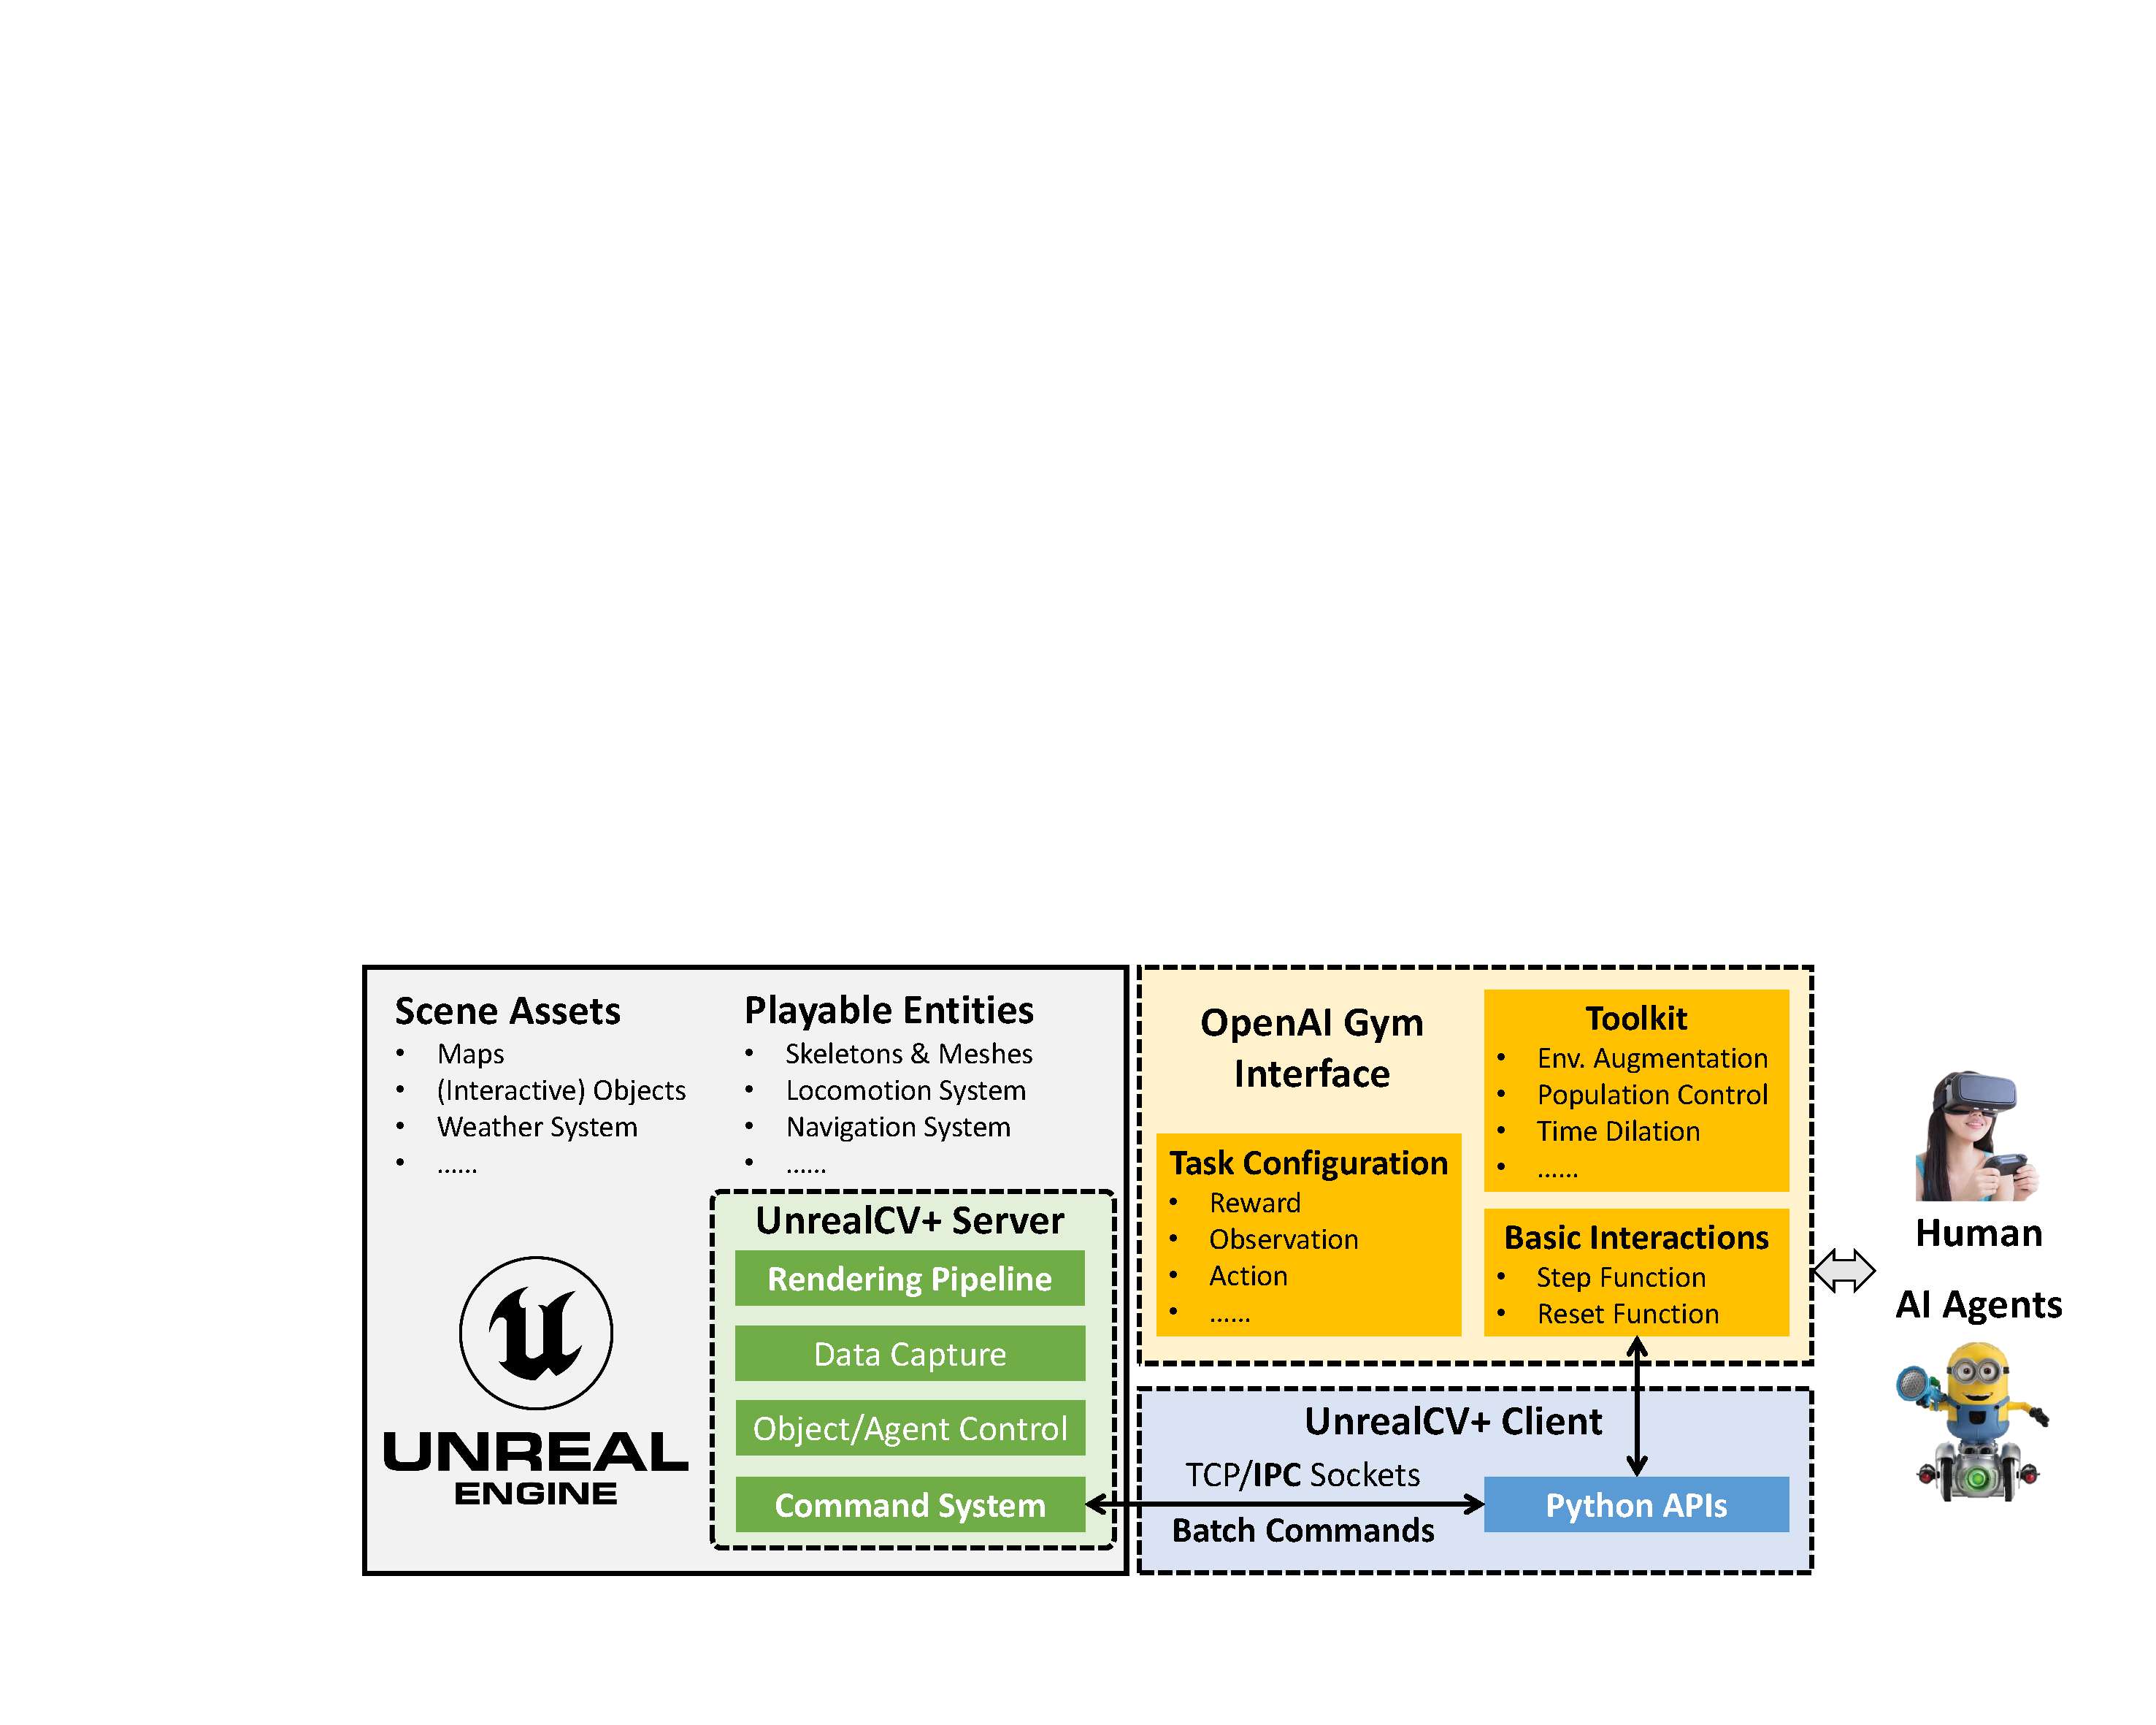
\includegraphics[width=0.99\textwidth]{image/architecture2.pdf}
    \caption{The detailed architecture of UnrealZoo. The Gray box indicates the UE binary, collecting the scenes and playable entities. The UnrealCV+ Server is built in the binary as a plugin. We have bolded the names of the optimized or new modules in UnrealCV+ Server and Client. We provide OpenAI Gym Interfaces for agent-environment interaction, which has been widely used in the community. Our gym interface supports customizing the task in a configuration file and contains a toolkit with a set of gym wrappers for environment augmentation, population control, etc.}
    \label{fig:architecture}
\end{figure}

We have tagged the collected scenes with several feature labels allowing researchers to select appropriate scenes for testing or training based on the tags associated with each scene. Our tags cover the following aspects:
\begin{itemize}
    \item \textbf{Scene Categories}: We categorize scenes into three main types: interior, exterior, and both. The interiors include private houses, museums, supermarkets, train stations, factories, gyms, and caves. The exteriors include various outdoor terrains such as ruins, islands, plazas, neighborhoods, and mountains. Additionally, there are 46 scenes that include both interior and exterior elements, offering a blend of architectural elements and natural landscapes, enhancing the versatility and realism of our collection. More details about the distribution of the scenes are shown in Figure~\ref{fig:stastic_distribution}.
    \item \textbf{Scale}: Each scene is labeled according to its scale, and categorized into four levels: indoor, building, community, and landscape. The indoor scale is the smallest, typically encompassing one or multiple interior rooms (up to a complete floor), such as apartments and office interiors. The building scale includes a single building and its immediate surroundings, like a museum, supermarket, or gas station. The community scale covers areas with multiple buildings, such as neighborhoods, villages, castles, or container yards. The landscape scale includes vast natural or man-made areas, or parts of a city or an entire small town, such as mountains, forests, islands, and urban districts.
    Specifically, there are 35 scenes classified as landscape, 28 as community, 23 as building, and 15 as indoor. The largest scene covers 16 square kilometers.
    % These combined scenes provide a comprehensive environment for studying the interactions and transitions of agents in complex spatial structures.
    % 24 interior only, 30 exterior, 46 exterior & interior
    \item \textbf{Spatial Structure}: 
    We also tag the spatial structure of the scenes, including multi-floor, topological, flat, steep, etc. Such categorization is vital for benchmarking the spatial intelligence of embodied agents. Multi-floor structures, for instance, challenge agents with vertical navigation and require advanced path-planning algorithms. Topological features, such as interconnected pathways, test the agent's ability to understand and traverse complex networks.
    \item \textbf{Dynamics}: The environment's dynamics include simulating factors like weather,  fire, gas, fluid, and interactive objects. These elements enhance the visual and physical diversity of the scene while evaluating agents' adaptability and generalization. Weather variations such as sandstorms, snowfall, and thunderstorms are crucial, as are interactive objects like doors that agents can interact with. These dynamics are vital for an open-world experience.
    \item \textbf{Style}: The scenes may also represent diverse styles that reflect various cultures and eras, such as \emph{Asian Temple}, \emph{Western Church}, and \emph{Middle Eastern Street}. Cultural labels include \emph{Western}, \emph{Asian}, and \emph{Middle Eastern}, while era labels encompass \emph{Medieval}, \emph{Modern}, and \emph{Science Fiction}. Identifying the styles will help us build a new data set to benchmark how social agents adapt to different backgrounds.
\end{itemize}

After categorizing the scenes, we integrate UnrealCV+ (Refer to Section~\ref{sec:unrealcv}) into the UE project and add the controllable player assets (Refer to Section~\ref{sec:body}) to each scene. Due to licensing restrictions, content purchased from the marketplace cannot be open-source, so we package the projects into an executable binary for sharing with the community. These executable binaries will be compatible with various operating systems, including Windows, Linux, and macOS, allowing users to download and run them via the Python interface without needing any knowledge of Unreal Engine, which is primarily built on C++ and Blueprint.

% This system can be used for non-player behavior control, demonstration trajectory collection,etc. For example, in a neighborhood environment, researchers can place multiple human and animal agents and publish random walking commands to simulate dense crowd scenarios, which can be used to train or evaluate embodied visual tracking tasks, as shown in the Figure. \ref{}. 


\subsection{Playable Entities}
\label{sec:body}
% functions/features for the agents
% hetergenous, diverse, interactable

UnrealZoo includes seven types of playable entities: humans, animals, cars, motorbikes, drones, mobile robots, and flying cameras (See Figure~\ref{fig:overview}). Specifically, it comprises 19 human entities, 27 animal entities (dog, horse, elephant, pig, bird, turtle, etc), 3 cars, 14 quadruped robots, 3 motorcycles, and 1 quad-copter drone. This diversity, with varying affordances like action space and viewpoint, allows us to explore new challenges in embodied AI, such as cross-embodiment generalization and heterogeneous multi-agent interactions.


\begin{figure}[b]
    \centering
    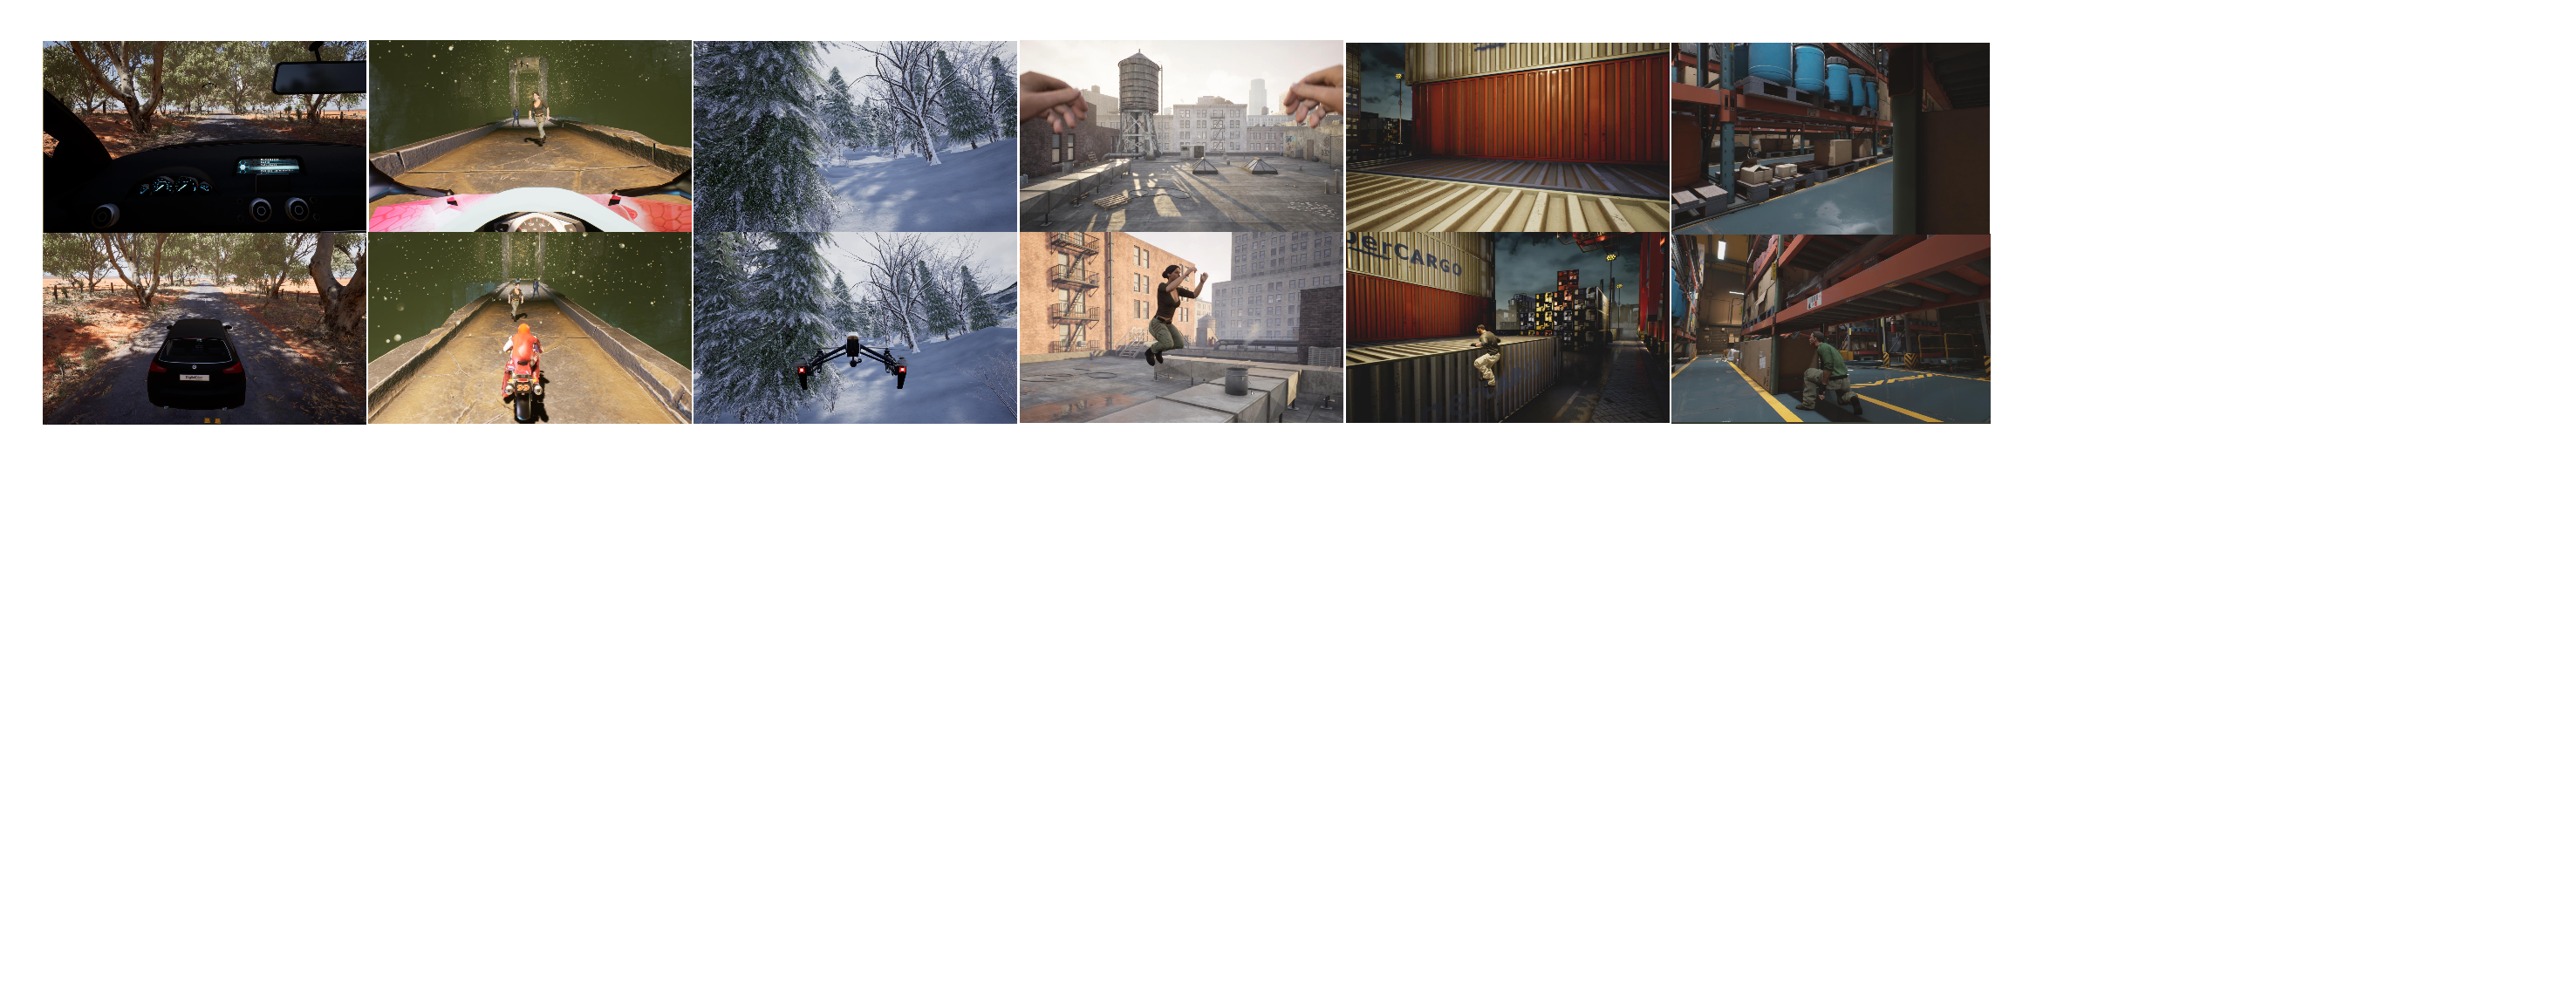
\includegraphics[width=0.99\textwidth]{image/body.pdf} 
    \caption{First-person (Top) and third-person (Bottom) view images of different entities in different scenes. Note that camera parameters can be reconfigured by UnrealCV APIs.}
    \label{fig:body}
\end{figure}

Each entity includes a skeleton with appropriate meshes and textures, a local motion system, and a navigation system.
We offer a set of callable functions for each entity, enabling users to modify attributes like size, appearance, and camera positions, as well as control movements. 
Each entity can switch between different textures and appearances via UnrealCV API, enhancing visual diversity and adaptability for various scenarios. 
Each entity is equipped with an ego-centric camera, allowing the users to capture various types of image data such as RGB, depth, surface normal, and instance-level segmentation (object mask) from the agent's ego-centric view. Figure~\ref{fig:body} shows examples of the captured first-person view and third-person view images of different entities with varying locomotion.
For multi-agent interaction, the population of the entities in a scene can be easily adjusted using the spawn or destroy functions. 

\textbf{The locomotion system} is built on \href{https://www.unrealengine.com/marketplace/en-US/product/smart-locomotion}{Smart Locomotion}, a well-designed and smooth locomotion system.
It contains a number of high-quality animations that enable the agent to interact with the scene, such as opening and closing doors, crouching under obstacles, jumping over obstacles, climbing onto a platform, and simulating injury or death. With the locomotion system, we can explore the agent's ability to reason, plan, and interact in large-scale complex 3D scenes in advance, ignoring learning skills for low-level action control that requires high-fidelity physical simulation.

\textbf{The navigation system} is built on \href{https://dev.epicgames.com/documentation/en-us/unreal-engine/world-partitioned-navigation-mesh?application_version=5.4}{NavMesh} allowing agents to autonomously navigate with the built-in AI controller.
This includes path-finding and obstacle-avoidance capabilities, ensuring smooth and realistic movement throughout diverse terrains and structures.
For urban-style maps, we segment the roads to distinguish between pedestrian and vehicle pathways. When agents use the navigation system for autonomous control, they will navigate the shortest path based on the priority of the different areas. For example, pedestrians and animals will prioritize walking on sidewalks, while vehicles and motorcycles will prioritize driving on roadways. An example of the navigation area is shown in Figure~\ref{fig:nav_mesh}.


\subsection{Programming Interface}

\label{sec:unrealcv}
We provide UnrealCV+ as the basic application programming interface (API) on Python to capture data and control the entities and scenes, and provide an OpenAI Gym interface for general agent-environment interactions. The architectures of the programming interfaces are shown in Figure~\ref{fig:architecture}.

\textbf{UnrealCV+} is our improved version of the UnrealCV~\citep{qiu2017unrealcv} for high-throughput interactions. As the original version of UrnealCV primarily focuses on generating synthesis data for computer vision, the frame rates per second (FPS) are not optimized for real-time interactions.
We optimize the rendering pipelines in the UnrealCV server and the communication protocols between the server and the client to improve the FPS. Specifically, we enable parallel processing while rendering object masks and depth images, which can significantly improve the FPS in large-scale scenes.
For multi-agent interactions, we further introduce the batch commands protocol. In this protocol, the client can simultaneously send a batch of commands to the server, processing all the received commands and returning a batch of results. In this way, we can reduce the time spent on server-client communication. Since reinforcement learning requires extensive trial-and-error interactions for training, often running multiple environments on a computer, we introduce Inter-process communication (IPC) sockets instead of TCP sockets to improve the stability of the server-client communication under high loads. We benchmark the FPS performance in Table~\ref{tab:fps_image}. 
To enhance user-friendliness, we have developed high-level Python APIs that are built upon the command systems of UnrealCV. These APIs encapsulate all the request commands and their corresponding data decoders into a callable Python function. This approach significantly simplifies the process for beginners, allowing them to interact with and customize the environment using UnrealCV+.

\begin{table}[tb]
\centering

\caption{Comparison of FPS in Unreal Engine 4.27 with UnrealCV and UnrealCV+. The reported result is an average performance across 6 typical environments.}
 \resizebox{\textwidth}{!}{
\begin{tabular}{l|c c c c|c c c}
\hline
 & \multicolumn{4}{c|}{Image Capture} & \multicolumn{3}{c}{Multi-agent Interaction} \\ % \cline{2-8} 
    & Color & Object Mask & Surface Normal & Depth & N=2 & N=6 & N=10 \\ \hline
UnrealCV  & 74 &70 & 109&52 & 35  & 13 & 8 \\ \hline
UnrealCV+  & $83(\uparrow12\%)$ & $154(\uparrow120\%)$ & $131(\uparrow20\%)$ & $97(\uparrow86\%)$ & $54(\uparrow54\%)$ & $25(\uparrow92\%)$ & $16(\uparrow100\%)$ \\ \hline
\end{tabular}
}
\label{tab:fps_image}
\vspace{-0.3cm}
\end{table}

\textbf{Gym Interface} is used to define the interactive tasks and standardize the agent-environment interaction, following \href{https://github.com/zfw1226/gym-unrealcv}{Gym-UnrealCV}.
Even though there are a lot of tasks for agents, they usually share common interaction protocols, i.e., the agent gets observations from the environment and returns actions. The main difference across different tasks usually is the reward functions, the modality of the observation, and the available actions. Hence, we define the basic interaction functions for general usage and list the task-specific configurations, e.g., scene name, and reward function, in a JSON File, as shown in Figure~\ref{app:json}. In this way, when adding new UE scenes, the users only need to set the parameters in the JSON files. Moreover, we contain a toolkit with a set of gym wrappers for training and testing the agents, such as environment augmentation that has been in previous work for training generalizable agents~\citep{luo2018end, luo2019pami}, population control to adjust the number of agents in the scene, and time dilation to adjust the control frequency in dynamic scenes. In Section~\ref{sec:social_tracking}, we demonstrate an example usage of the toolkit to analyze the robustness of social tracking agents to the population of crowds and the impact of the control frequency in such dynamic scenes. We also provide a launch tool to enable the user to run multiple environments with specific GPU IDs within a computer, which is useful for distributed online reinforcement learning~\citep{ci2023proactive}.


\vspace{-0.3cm}
\section{Experiments}
\vspace{-0.3cm}
In this section, we use a subset of UnrealZoo to demonstrate the usability of the collected environments. For visual navigation, we select two scenes with complex spatial structures to train and validate the RL-based and VLM-based agents.
For active tracking, we select at most 8 scenes as training environments and validate the generalization of the learned policy in another 24 scenes, which are divided into four categories according to the scene types. The results demonstrate the importance of the diversity of the training environments to the cross-domain generalization.
For social tracking, we analyze the robustness of the agent in social environments with different control frequencies, using the toolkit provided in the gym to generate crowds with varying populations and control frequencies.

\vspace{-0.2cm}
\subsection{Visual Navigation} 
\vspace{-0.2cm}

visual navigation in the wild introduces a new level of complexity compared to traditional navigation tasks for indoor scenes or autonomous driving, which often run on complex 3D spatial structures. 
Differently, we place the agent in open-world environments where it must take a set of locomotion, e.g., running, climbing, jumping, crouching, to go over the various obstacles in unstructured terrains to reach the target object. In this setting, the agent requires advanced spatial reasoning and actions to make real-time decisions about its path. 
The emphasis on such complex environments ensures the agent can operate effectively in a broad range of challenging scenarios, moving beyond the constraints of traditional navigation frameworks. The details of the task setting are introduced in Appendix~\ref{app:navigation_task}.

\textbf{Evaluation Metrics.}
We employ two key metrics to evaluate visual navigation agents: 1) Average Episode Length (EL), representing the average number of steps per episode over 50 episodes. 2) Success Rate (SR), measuring the percentage of episodes the agent successfully navigates to the target object out of 50 total episodes, which represents the navigation capability in the wild environment.

\textbf{Baselines for Navigation.} We build simple baselines to demonstrate the applicability of our environments for training reinforcement learning agents and benchmark the agents based on pre-trained large models.
\textbf{1) Online RL}: We trained the RL-based navigation agents separately in the Roof and Factory environments using a distributed online reinforcement learning (RL) approach, e.g. A3C~\citep{mnih2016asynchronous}. The training curve is shown in Figure~\ref{fig:training_curve}. The model takes the first-person view segmentation mask and the relative position between the agent and target as input, and outputs direct control signals (from the predefined action space) to navigate. This setup allows the agent to learn and optimize navigation strategies during continuous interaction with the environment. Please refer to Appendix~\ref{app:onlineRL} for the implementation details.
\textbf{2) GPT-4o}: We employ the GPT-4o model to take action, leveraging its powerful multi-modal reasoning capabilities. The model takes first-person view images and the relative position between the agent and the fixed target as input. The GPT-4o model follows our prompt template (See Table~\ref{app:prompt_navigation}) as guidance, reasoning appropriate actions from the predefined control space to guide the agent toward the target.
\textbf{3) Human}: We also have a human player control the agent using a keyboard, similar to a first-person video game. The player navigates the agent from a random starting point to a fixed target, making decisions based on visual observations from the shared control space.

\textbf{Results.}
In Table~\ref{tab:nav_res}, we report the performances of different methods in two unstructured scenes. The RL-based agent performs moderately well, achieving better results in the simpler environment (\emph{IndustrialArea}) compared to the \emph{Roof}, where the target object is located on different levels of stairs. The GPT-4o agent struggles in both scenarios. This infers that the GPT-4o performs poorly in complex 3D scene reasoning. As a reference, the human player completes both tasks with the fewest steps and a 1.00 success rate, underscoring the significant performance gap between current embodied AI agents and humans, indicating substantial room for improvement to navigate in such complex, open-world environments.

\begin{wraptable}{r}{0.47\textwidth}
\vspace{-0.2cm}
\centering
\caption{The results (EL/SR) of visual navigation in two unstructured terrains. }
\begin{tabular}{c|cc}
\hline
\bf Methods & \bf Roof & \bf IndustrialArea \\  
\hline 
Online RL & 1660/0.32 & 261/0.52 \\  
GPT-4o & 2000/0.00 & 369/0.20 \\  
\hline
Human & 515/1.00 & 158/1.00 \\  
\hline
\end{tabular}
\label{tab:nav_res}
\end{wraptable}

\begin{figure}
    \centering
    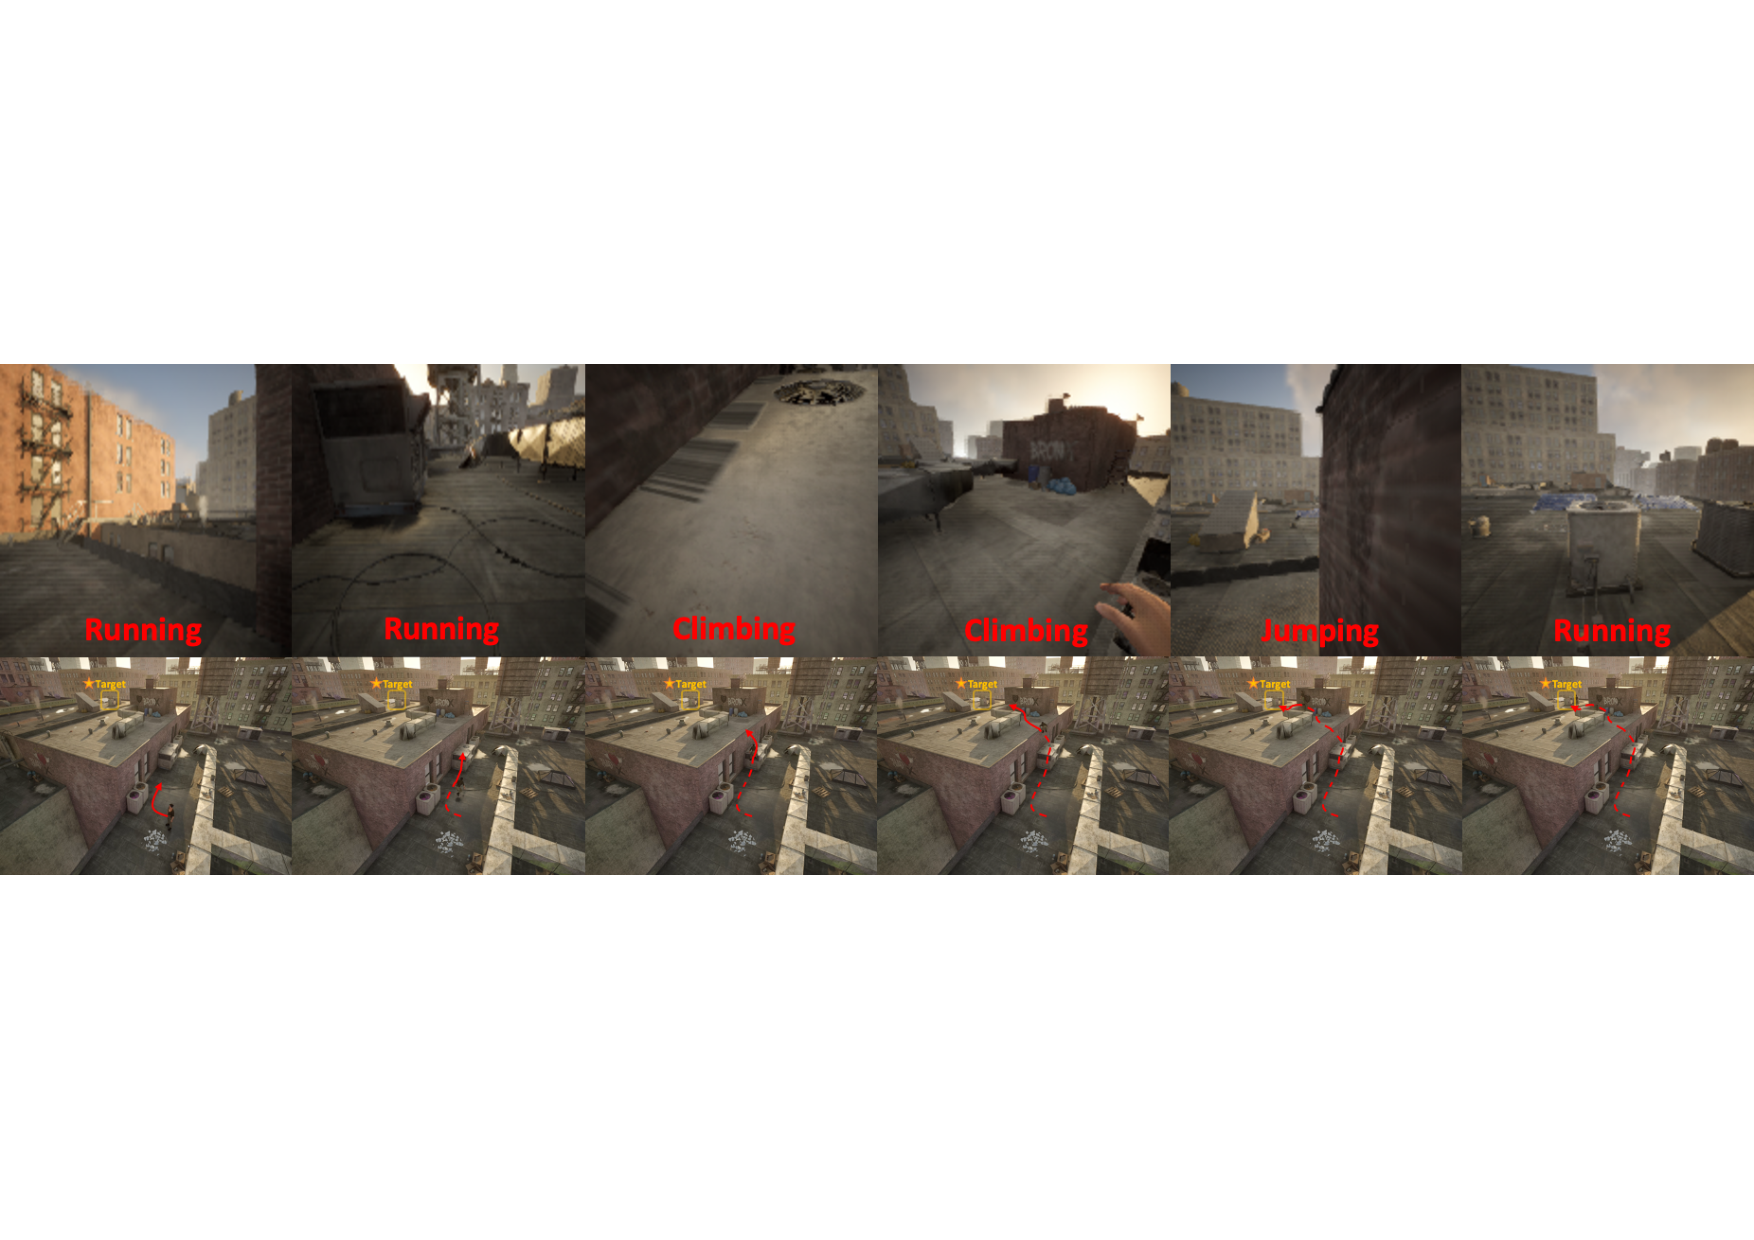
\includegraphics[width=0.99\linewidth]{image/vis2.pdf}
    \caption{An exemplar sequence from the embodied navigation agent in the \emph{Roof}. The RL-based agent learned to climb on a box and wall and jump over an obstacle to reach the goal location in a short path.}
    \label{fig:eval_example}
    \vspace{-0.5cm}
\end{figure}

\subsection{Active Visual Tracking}

We evaluate the generalization of the tracking agents across four environment categories: \textbf{Interior Scenes}, \textbf{Palaces}, \textbf{Wilds}, and \textbf{Modern Scenes}. 
Each category contains 4 individual environments, as shown in Figure ~\ref{fig:eval_env}.
We aim to capture a broad range of features in our environment collection by selecting four distinct and representative scenes from each category, ensuring a comprehensive evaluation of the agents' capabilities. The details of the tasks are introduced in Appendix~\ref{app:tracking_task}. We analyzed the effectiveness of the diversity of the training data by collecting demonstrations with different numbers of training environments.


\textbf{Evaluation Metrics.}
Our evaluation employs three key metrics: (1) Average Episodic Return (ER), which calculates the mean episodic return over 50 episodes, providing insights into overall tracking performance; (2) Average Episode Length (EL), representing the average number of steps per episode, which reflects long-term tracking effectiveness; and (3) Success Rate (SR), measuring the percentage of episodes that complete 500 steps out of 50 total episodes. 

 
\textbf{Baselines for Active Visual Tracking.}
For the \emph{RL-based agents}, we extend from the official implementation settings from the recent offline RL method \citep{zhong2024empowering}, collecting offline datasets and employing the original network architecture. 
To demonstrate the impact of data diversity on tracking performance, we collect three sets of offline datasets, each containing 100k steps. The key difference between these datasets is the number of environments used for data collection: one was collected in a single environment (denoted as \textit{1 Env.}), another in two environments(denoted as \textit{2 Envs.}), and the third in eight distinct environments (denoted as \textit{8 Envs.}). The offline training curve of each setting is shown in Figure~\ref{fig:offline_curve}. The environment distribution of each dataset setting is shown in Figure~\ref{fig:data_distribution}. It is worth noting that \underline{FlexibleRoom}, one of the environments used for data collection, is a unique abstract environment, with all objects represented as geometric shapes covered by randomized patterns. This distinctive setup contrasts with the more realistic and diverse environments in the collection, offering a unique scenario for testing agent adaptability. 
For the \emph{VLM-based agents}, we utilize the latest large models GPT-4o to directly generate actions based on observed images for tracking a target person. To ensure smooth and precise transitions, we designed a system prompt that helps the model understand the task while standardizing the output format to align with predefined action settings. This prompt ensures the model produces actions coherent with the task's requirements. Specifically, GPT-4o is tasked with generating concrete action decisions from a predefined instruction space: moving forward, moving backward, turning left, turning right, or maintaining the current position. Once an instruction is generated, we map it to corresponding linear and angular velocities to update the agent's movement in the environment. It is important to note that while the system prompt can use raw image observations as input, our experience shows poor alignment performance and significant time delays, which pose challenges for real-time tracking. The full system prompt and mapping relationship are provided in Appendix~\ref{app:prompt}.



% \subsubsection{Experiment result}
\textbf{Result Analysis.}
We first evaluate the performance of agents trained with offline datasets collected from varying numbers of environments (1 Env., 2 Envs., 8 Envs.) across \textbf{16 distinct environments}. We list the detailed evaluation results across the entire 16 environments in Table~\ref{tab:eval_res}. To better visualize the performance change of different training settings within various scene categories, we calculate the average success rate (SR) of each agent in four categories, the results are shown in Figure~\ref{fig:eval_SR}. The results reveal a clear trend: \textbf{as the number of environments used for training increases, agent long-term tracking performance generally improves across all categories.} In the Wilds, a significant increase in success rate is observed with the 8 Envs. dataset, which involves the highest diversity of environments. This demonstrates that diverse environmental exposure plays a crucial role in improving the agent's generalization capabilities in more complex, open-world environments. The lower success rate in the 1 Env. dataset highlights the limitations of training solely in abstract settings like the FlexibleRoom. Similarly, in the Palace, the success rate improves notably from 1 Env. to 8 Envs., suggesting that training with a broader range of environments helps the agent better adapt to intricate spatial structures typical of Palace-like maze environments.

\begin{wrapfigure}{r}{0.5\textwidth}
%\vspace{-1.5cm}
    \centering
        \vspace{-0.7cm}
    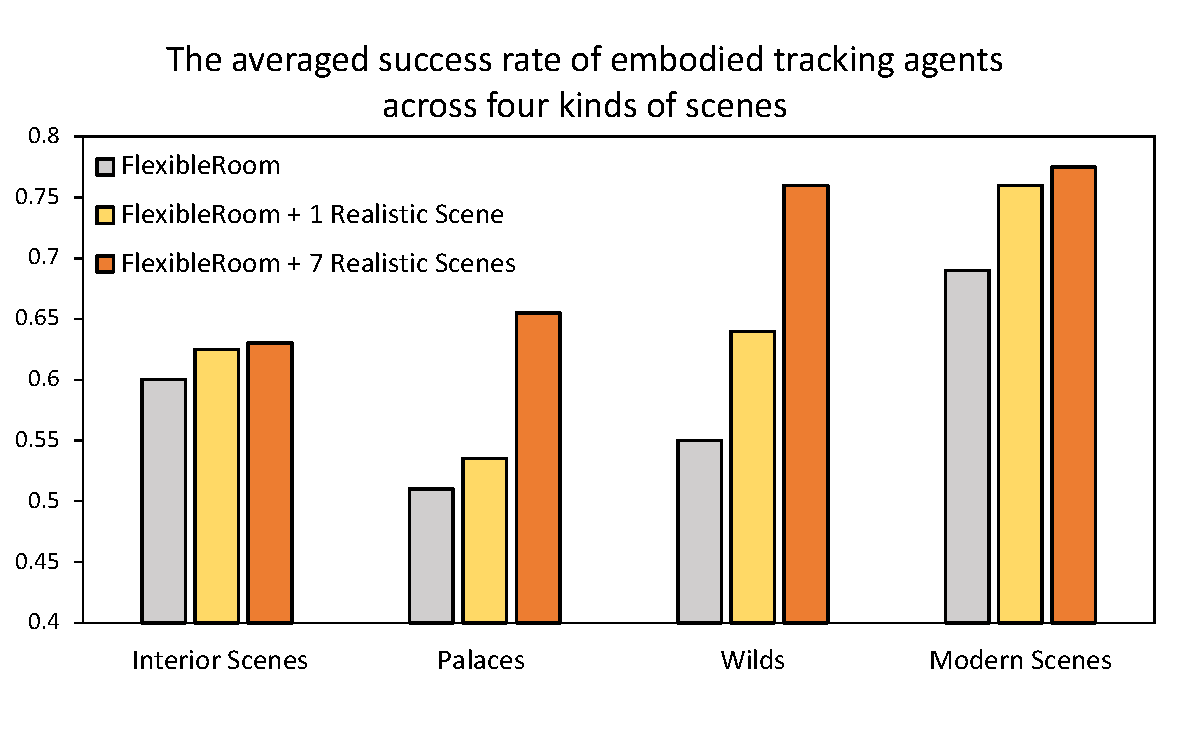
\includegraphics[width=\linewidth]{image/SR_performance.pdf}
    \caption{Average success rate of agents across four environment categories: Compact Interior, Wildscape Realm, Palace Maze, and Lifelike Urbanity, evaluated under three offline dataset settings (1 Env, 2 Envs., 8 Envs.). The results show the generalization capability improves significantly as more diverse environments are included in the dataset. However, environments with complex spatial structures, such as Compact Interior and Palace Maze, exhibit lower success rates, highlighting challenges in obstacle avoidance and navigation.}
    \vspace{-0.4cm}
    \label{fig:eval_SR}
\end{wrapfigure}

\vspace{-0.2cm}
\subsection{Social Tracking}
\vspace{-0.2cm}
\label{sec:social_tracking}
We further evaluate the tracking agents in a social scenario, where the agent needs to follow the target in crowds. Such a setting contains varying high-dynamics objects with similar appearances, e.g., pedestrians. We can directly apply the population control wrapper in the Gym toolkit to extend the environment used for active tracking to this setting.

\textbf{Robustness to Active Distractions.}
A key challenge in active visual tracking tasks is managing active distractions, a critical issue for real-world deployment in crowds. 
Thus, we conducted an experiment in the \emph{DowntownWest} and generated crowds with varying numbers of human characters as distractors notated as 4D, 8D, and 10D. The number indicates the number of distractors. We compared the performance of the offline RL method, trained under three dataset configurations (1 Env., 2 Envs., 8 Envs.), against the VLM-based method, evaluating the agents’ ability to maintain robust tracking under these different levels of active distractions.

The results in Table~\ref{tab:eval_robust} show clear performance differences between the offline RL methods (1 Env., 2 Envs., 8 Envs.) and the GPT-4o model in handling active distractions. As the number of distractors increases, the offline RL methods maintain relatively stable success rates (SR), with the highest performance seen in the 8 Envs. setting, which achieves an SR of 0.8 in the 4D condition and remains robust with slight declines in the 8D and 10D conditions (0.72 and 0.68, respectively). This suggests that the agent benefits from the richer diversity of training data, enabling it to handle increasingly complex crowd scenarios more effectively.
On the other hand, the GPT-4o model consistently struggles with active distractions, showing significantly lower average returns (ER) and success rates across all settings. The model's inability to cope with dynamic, crowded environments is evidenced by its poor performance, particularly in the 10D condition where it records a success rate of just 0.1. This highlights a major limitation of the VLM-based method in dynamic environments with active distractions, as it lacks the temporal consistency and real-time adaptability required for effective tracking. Further evaluation results across different environments are provided in the Appendix~\ref{app:social}.

\textbf{Cross-Embodiment Generalization.} We transfer the agent trained for the human character to the robot dog, which observes the world from a lower perspective. We can see that the results in Table~\ref{tab:eval_robust} drop, particularly the success rate, indicating that the research community should pay more attention to the cross-embodiment generalization.

\textbf{The Impact of Control Frequency.} 
We employ the time dilation wrapper to simulate different control frequencies during deployment. The frequency of the perception-control loop is crucial for handling dynamic environments. As is shown in Table~\ref{tab:frequency_control}, when the rate drops below 10 FPS, performance significantly declines.
We observe that higher control frequencies enable RL-based agents to perform better in social tracking. These results emphasize the importance of building efficient models for embodied agents, to accomplish tasks in dynamic open worlds.

\begin{wraptable}{r}{0.35\textwidth}
    \centering
    \vspace{-0.5cm}
        \caption{The impact of control frequency on tracking performance. We evaluate the agent (Offline RL 1 Env.) in the \underline{FlexibleRoom} environment using the time dilation wrapper to simulate varying control frequencies.}
    \begin{tabular}{c|c} 
    \hline
        & ER/ EL/ SR. \\ \hline
        3 FPS &184/377/0.34  \\ 
        10 FPS &303/449/0.62 \\ 
        30 FPS &368/482/0.92 \\ \hline
        w/o Control & 275/425/0.74 \\ \hline
    \end{tabular}
    \label{tab:frequency_control}

\end{wraptable}

\begin{table}[tb]
    \centering
    \caption{Performance comparison of different methods in the \underline{DowntownWest} environment with varying numbers of distractors (4D, 8D, 10D). Each cell presents three metrics from left to right: Average Episodic Return (ER), Average Episode Length (EL), and Success Rate (SR). }
    \vspace{-0.2cm}
\begin{tabular}{c|ccc}
\hline
%\toprule
      Method  & \tabincell{c}{4D} &  \tabincell{c}{8D} &  \tabincell{c}{10D} \\ \hline
%\midrule
Offline RL 1 Env. & 251/450/0.70 & 201/406/0.58 &  230/247/0.64 \\
Offline RL 2 Envs. & 309/456/0.74 & 259/424/0.68 &  258/428/0.68 \\
Offline RL 8 Envs. &245/458/0.80&225/435/0.72&218/444/0.68 \\
Offline RL 8 Envs. (Robot dog) &220/409/0.48 & 189/386/0.42 & 143/367/0.40\\
GPT-4o & -102/264/0.16&-64/270/0.14	&-80/240/0.10 \\
\hline
%\bottomrule
\end{tabular}
    % \end{threeparttable}
    % }
    \vspace{-0.5cm}
    \label{tab:eval_robust}
\end{table}

% GPT-4o, CoELA
\vspace{-0.1cm}
\subsection{Limitation Analysis and Summary}
\vspace{-0.1cm}
The current RL method shows some capacity to learn spatial-temporal information and dynamically respond to target movement in most scenarios, but it struggles with executing advanced actions like bypassing obstacles. In compact Interior categories and some special environments such as \underline{TerrainDemo}, \underline{IndustrialArea}, and \underline{ModularSciFiSeason1}, which feature irregular landscapes, narrow passageways, and maze-like structures, the agent often collides with casually placed low-level objects. While the agent can track targets, it's insufficient to handle unpredictable hindrances, especially in key moments like bypassing corners or tight spaces, which increases the likelihood of failure. This highlights a significant limitation: although the agent can learn and react to its environment, it lacks the higher-level reasoning to anticipate and avoid obstacles effectively. Advanced behaviors like bypassing obstacles are crucial for improving performance, especially in cluttered environments where basic reactive controls are insufficient. Incorporating such reasoning mechanisms would help reduce failure rates, particularly in critical scenarios, and improve overall tracking performance.

For the VLM-based method, one key factor contributing to GPT-4o's notably poor performance, especially in comparison to the RL methods, is its susceptibility to time delays. From our experience, this issue becomes particularly evident when the target makes abrupt movements, such as turning around. Due to the API's response lag, the GPT-4o agent struggles to track the target in real time, often losing it before receiving updated instructions. This limitation highlights the difficulty of real-time processing in embodied tracking tasks using models that rely on slower external API communications, underscoring the need for more efficient integration methods for such systems.

\vspace{-0.3cm}
\section{Conclusions}
\vspace{-0.3cm}
In conclusion, we present UnrealZoo, a versatile platform designed to advance embodied AI research.
The diversity and complexity of the collected realistic environments challenge agents with varying embodied interaction tasks, such as visual navigation, active tracking across various environments, and social tracking in crowds. The enhanced UnrealCV+ API supports efficient data collection and task customization, enabling seamless interaction for both single and multi-agent systems. These features will open up potential applications like developing spatial intelligence in the 3D world and social intelligence in human-AI society, making our platform a valuable tool for pushing the boundaries of embodied AI in real-world scenarios. Looking forward, we will continue to enrich the virtual worlds with diverse scenes, bodies, and interaction tasks, advancing agents from the virtual realm to reality for a harmonious human-AI society.


\textbf{Limitations.} While our proposed environment provides diverse and complex scenarios for visual navigation, tracking, and other visual-based tasks, it currently lacks high-fidelity physical simulation, limiting the agent's ability to manipulate objects. Additionally, transferring learned behaviors to different embodied agents poses a challenge, as adapting models to various physical structures and control schemes is not yet seamless. These issues highlight areas for further research to enhance interaction dynamics and improve generalization across diverse agent embodiments.

\section*{Acknowledgements}
This work was supported by the National Science and Technology Major Project (2022ZD0114904), NSFC-6247070125, NSFC-62406010, the State Key Lab of General Artificial Intelligence at Peking University, and Qualcomm University Research Grant. We express our gratitude to Weichao Qiu for his invaluable support in optimizing UnrealCV and for the insightful discussions. We are also thankful to Tingyun Yan for providing the early version of the human entity and to Jingzhe Lin for his assistance in producing demo videos. Our appreciation extends to the active developers in the open-source community for ensuring UnrealCV's compatibility with the latest Unreal Engine versions, such as UE 5.4. Furthermore, we thank the contributors in the Unreal Engine Marketplace for offering high-quality content and plugins, which have been instrumental in the development of UnrealZoo.

\bibliography{reference}
% \bibliographystyle{plainnat}
\bibliographystyle{iclr2025_conference}

%%%%%%%%%%%%%%%%%%%%%%%%%%%%%%%%%%%%%%%%%%%%%%%%%%%%%%%%%%%%
\clearpage
\appendix
\appendix

% \section{Claimed Emergent Abilities}
% \label{app:claimed_emergent_abilities}

% We compile the models, tasks and metrics that different papers have claimed reveal emergent abilities of large language models. This list may be incomplete or inaccurate, but represents a good faith attempt to compile this information. Note: quantifying model scale when an ability emerges is complicated by the fact that different papers report model scale differently, either as (a) number of parameters \cite{brown2020language, ganguli2022predictability}, (b) effective number of parameters \cite{srivastava2022beyond} or (c) training FLOPs \cite{wei2022emergent}.

% \begin{table}[h!]
%     \centering
%     \begin{tabular}{|l|c|c|c|}
%     \hline
%         Task & Model Families & Metric & Model Scale at Emergence \\
%         \hline
%         2-Digit Addition \cite{brown2020language} & GPT-3 & Accuracy & 13B Parameters\\
%         2-Digit Subtraction \cite{brown2020language} & GPT-3 & Accuracy & 13B Parameters\\
%         3-Digit Addition \cite{brown2020language, ganguli2022predictability} & GPT-3 & Accuracy & 175B Parameters\\
%         3-Digit Subtraction \cite{brown2020language} & GPT-3 & Accuracy & 175B Parameters\\
%         MMLU \cite{ganguli2022predictability} & GPT-3, Gopher & Accuracy & 200B, 300B Parameters\\
%         Program Synthesis \cite{ganguli2022predictability} & Google Internal & \% Samples Solving Task & 200B Parameters\\
%         Figure of Speech Detection \cite{srivastava2022beyond} & ? & ? & $\sim 10^{11}$ Effective Parameters \\
%         IPA Transliterate \cite{srivastava2022beyond, wei2022emergent} & LaMDA, GPT-3 & BLEU & $\sim 10^{23}, \sim 10^{23}$ Training FLOPs\\
%         Periodic Elements \cite{srivastava2022beyond} & ? & ? & ?\\
%         Modified Arithmetic \cite{srivastava2022beyond, wei2022emergent} & GPT-3, LaMDA & Accuracy & $\sim 10^{23}, \sim 10^{24}$ Training FLOPs\\
%         Repeat Copy Logic \cite{srivastava2022beyond} & ? & ? & $10^{11}$ Effective Parameters\\
%         Word Unscrambling \cite{srivastava2022beyond, wei2022emergent} & LaMDA & Exact Match & $\sim 10^{24}$ Training FLOPs\\
%         Persian QA \cite{wei2022emergent} & PaLM & Exact Match & $\sim 10^{24}$ Training FLOPs\\
%         Truthful QA \cite{wei2022emergent} & Gopher & Accuracy & $\sim 10^{23}$ Training FLOPs\\
%         Grounded Mappings \cite{wei2022emergent} & ? & ? & ?\\
%         Multi-task NLU \cite{wei2022emergent} & ? & ? & ?\\
%         Word in context \cite{wei2022emergent} & ? & ? & $\sim 10^{24}$ Training FLOPs\\
%         \hline
%     \end{tabular}
%     \newline
%     \caption{\textbf{Tasks, model families, metrics and number of parameters for emergent abilities.}}
%     \label{tab:my_label}
% \end{table}


% \section{Exponentiated Negative Cross Entropy Lower Bounds Accuracy}
% \label{app:acc_bound}

% Consider batch size $B$ with length $L$. During training i.e. with teacher-forcing, the per-token accuracy (averaged over batch index $b$ and sequence index $l$) is defined as:
% %
% \begin{align}
%     \text{Acc} &\defeq \frac{1}{B} \sum_b \frac{1}{L} \sum_l p(t_{bl}^* | t_{b, <l}^*)\\
%     &= \frac{1}{BL} \sum_{b, l} p(t_{bl}^* | t_{b, <l}^*)
% \end{align}

% The cross entropy (commonly averaged over the batch) is defined as:
% %
% \begin{align}
%     \mathcal{L}_{CE} &\defeq -\frac{1}{B} \sum_b \log p(t_{b 1}^*, ..., t_{b L}^*)\\
%     &= -\frac{1}{B} \sum_b \log \prod_l p(t_{b l}^*| t_{b, <l}^*)\\
%     &= -\frac{1}{B} \sum_{b, l} \log p(t_{bl}^* | t_{b, <l}^*)
% \end{align}

% To make the comparison between accuracy and cross entropy a little easier, let's normalize the cross entropy by the sequence length:
% %
% \begin{align}
%     \mathcal{L}_{CE/L} &\defeq \frac{1}{L}\mathcal{L}_{CE}\\
%     &=  -\frac{1}{BL} \sum_{b, l} \log p(t_{bl}^* | t_{b, <l}^*)
% \end{align}

% Recall that Jensen's inequality tells us that for any random variable $X$, $\log \mathbb{E}[X] \geq \mathbb{E}[\log X]$. The relationship between sequence-length-normalized cross entropy and accuracy is thus:
% %
% \begin{align}
%     -\mathcal{L}_{CE/L} = \frac{1}{BL} \sum_{b, l} \log p(t_{bl}^* | t_{b <l}^*) &\leq \log \frac{1}{BL} \sum_{b, l}  p(t_{bl}^* | t_{b <l}^*) = \log \text{Acc}\\
%     \exp(- \mathcal{L}_{CE/L}) &\leq \text{Acc}
% \end{align}

% Consequently, we see that driving the cross entropy loss to $0$ necessarily drives the accuracy to $1$.

% TODO: Can we use the second moment method to derive bounds on how (un)likely a subset of tokens are to deviate from the mean?


\section{Approximate Behavior of Metrics on Sequential Data}
\label{app:metric_scaling}

How do different metrics behave when used to measure autoregressive model outputs? Precisely answering this question is tricky and possibly analytically unsolvable, so we provide an approximate answer here.

Notationally, we consider $N$ test data of length $L$ (here, length is measured in tokens) with targets denoted $t_n \defeq (t_{n1}, t_{n2}, ... t_{nL})$, the autoregressive model has a true-but-unknown per-token error probability of $\epsilon \in [0, 1]$ and the model outputs prediction $\hat{t}_n \defeq (\hat{t}_{n1}, \hat{t}_{n2}, ... \hat{t}_{nL})$. This assumes that the model's per-token error probability is constant, which is empirically false, but modeling the complex dependencies of errors is beyond our scope.

\subsection{Per-Token Error Probability is Resolution-Limited}
\label{app:metric_scaling:resolution_limited}

Note that because we have $N$ test data, each of length $L$, our resolution for viewing the per-token error probability $\epsilon$ is limited by $1/NL$. 
Here, resolution refers to ``the smallest interval measurable by a scientific instrument; the resolving power."
To explain what resolution means via an example, suppose one wants to measure a coin's probability of yielding heads.
After a single coin flip, only two outcomes are possible (H, T), so the resolution-limited probability of heads is either $0$ or $1$.
After two coin flips, four outcomes are possible (HH, HT, TH, TT), so the resolution-limited probability of heads is now one of $0, 0.5, 1$.
After $F$ coin flips, we can only resolve the coin's probability of yielding heads up to $1/F$.
Consequently, we introduce a resolution-limited notation:
%
\begin{equation}
    \nint{a}_b \defeq \text{$a$ rounded to the nearest integer multiple of $1/b$}
\end{equation}

\subsection{Token Edit Distance}
\label{app:metric_scaling:token_edit_distance}

We first consider an adaptation of the Levenshtein (string edit) distance for models that function on tokens rather than characters, an adaptation we term the \textit{token edit distance}. The token edit distance between two token sequences $t_n, \hat{t_n}$ is defined as the integer number of additions, deletions or substitutions necessary to transform $t_n$ into $\hat{t}_n$ (or vice versa).

\begin{align}
    \text{Token Edit Distance}(t_n, \hat{t}_n)  &\defeq \text{Num Substitutions} + \text{Num. Additions} + \text{Num. Deletions}\\
    &= \sum_{\ell =1}^L \mathbb{I}[t_{n\ell} \neq \hat{t}_{n\ell}] + \text{Num. Additions} + \text{Num. Deletions}\\
    &\geq \sum_{\ell =1}^L \mathbb{I}[t_{n\ell} \neq \hat{t}_{n\ell}]
\end{align}

The expected token edit distance is therefore:

\begin{align}
    \mathbb{E}[\text{Token Edit Distance}(t_n, \hat{t}_n)] &\geq \mathbb{E}[\sum_{\ell =1}^L \mathbb{I}[t_{n\ell} \neq \hat{t}_{n\ell}]]\\
    &= \sum_{\ell =1}^L p(t_{n\ell} \neq \hat{t}_{n\ell})\\
    &\approx L (1 - \epsilon)
\end{align}

The resolution-limited expected token edit distance is therefore:

\begin{equation}
    \nint{\mathbb{E}[\text{Token Edit Distance}(t_n, \hat{t}_n)]}_{NL} \geq L \Big(1 - \nint{\epsilon}_{NL} \Big)
\end{equation}

From this, we see that the expected token edit distance scales approximately linearly with the resolution-limited per-token probability. The real rate is slightly higher than linear because additions and deletions contribute an additional non-negative cost, but modeling this requires a model of how likely the model is to overproduce or underproduce tokens, which is something we do not currently possess.

\subsection{Accuracy}
\label{app:metric_scaling:accuracy}

\begin{align}
    \text{Accuracy}(t_n, \hat{t}_n) &\defeq \mathbb{I}[\text{No additions}] \, \mathbb{I}[\text{No deletions}] \, \prod_{l=1}^L \mathbb{I}[t_{nl} = \hat{t}_{nl}]\\
    &\approx \prod_{l=1}^L \mathbb{I}[t_{nl} = \hat{t}_{nl}]
\end{align}

As with the Token Edit Distance (App. \ref{app:metric_scaling:accuracy}), we ignore how likely the language model is to overproduce or underproduce tokens because we do not have a good model of this process. Continuing along,

\begin{align}
    \mathbb{E}[\log \text{Accuracy}] &= \sum_l \mathbb{E}[\log \mathbb{I}[t_{nl} = \hat{t}_{nl}]]\\
    &\leq \sum_l \log \mathbb{E}[\mathbb{I}[t_{nl} = \hat{t}_{nl}]]\\
    &\approx L \log (1- \epsilon)
    % \exp(\mathbb{E}[\log \text{Accuracy}]) &= \exp (\sum_l \mathbb{E}[\log \mathbb{I}(t_{nl}, \hat{t}_{nl})])\\
    % &=
\end{align}

Taking an approximation that would make most mathematicians cry:

\begin{align}
    \mathbb{E}[\text{Accuracy}] &\approx \exp(\mathbb{E}[\log \text{Accuracy}])\\
    &= (1 - \epsilon)^L\\
\end{align}

This reveals that accuracy \textbf{approximately} falls geometrically with target token length. The resolution-limited expected accuracy is therefore:

\begin{equation}
    \nint{\mathbb{E}[\text{Accuracy}]}_{NL} = \nint{(1 - \epsilon)^L}_{NL}
\end{equation}

From this we can see that choosing a nonlinear metric like Accuracy is affected significantly more by limited resolution because Accuracy forces one to distinguish quantities that decay rapidly.

\subsection{ROUGE-L-Sum}
\label{app:metric_scaling:rougeLsum}

\begin{figure}
    \centering
    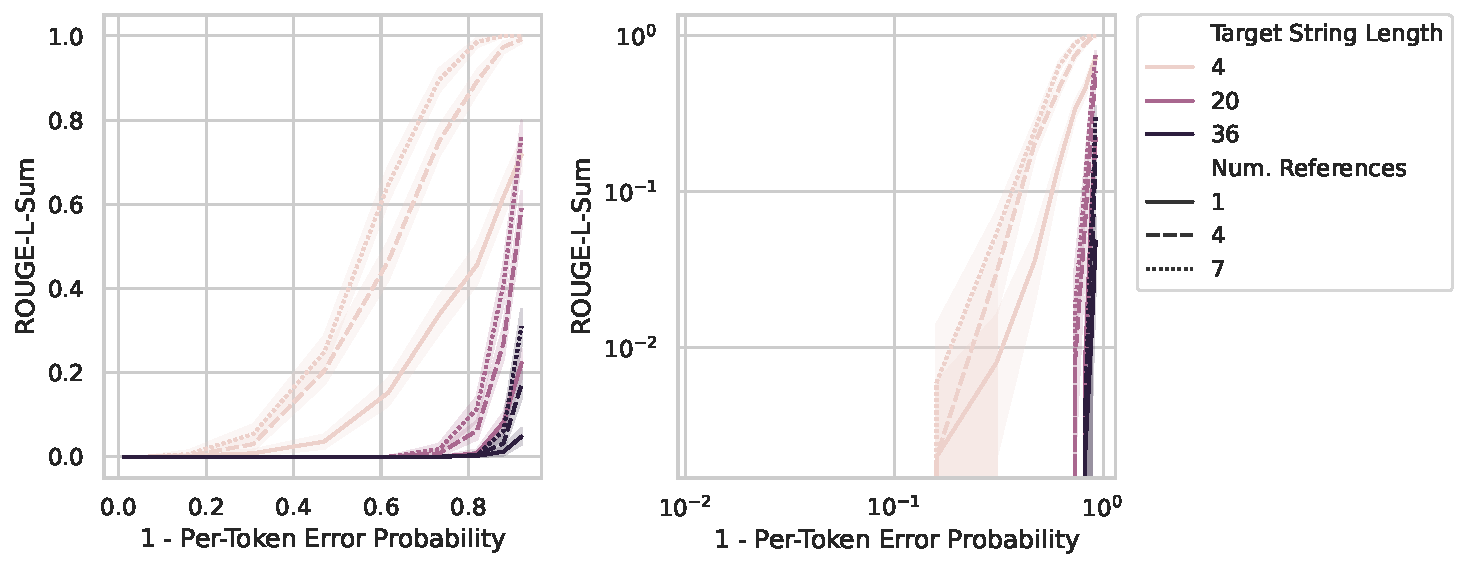
\includegraphics[width=0.95\textwidth]{figures/rouge_understanding/rougeLsum_vs_token_error_prob_scaling_simulation.pdf}
    \caption{\textbf{ROUGE-L-Sum is a sharp metric.} Simulations show that as the per-token error probability slightly increase (e.g. from 0.05 to 0.1), the ROUGE-L-Sum metric sharply falls.}
    \label{fig:app:metric_scaling:rougeLsum}
\end{figure}


Another BIG-Bench metric \cite{srivastava2022beyond} is ROUGE-L-Sum \cite{lin2004rouge}, a metric based on the longest common subsequence (LCS) between two sequences. Section 3.2 of \cite{lin2004rouge} gives the exact definition, but the key property is that ROUGE-L-Sum measures the ``union" LCS, which means ``stitching" together LCSs across the candidate and multiple references. As explained in the original paper: if the candidate sequence is $c = w_1 w_2 w_3 w_4 w_5$, and if there are two reference sequences $r_1 = w_1 w_2 w_6 w_7 w_8$ and $r_2 = w_1 w_3 w_8 w_9 w_5$, then $LCS(r_1, c) = w_1 w_2$ and $LCS(r_2, c) =w_1 w_3 w_5$, then the \textit{union} 
-LCS of $c, r_1, r_2$ is $w_1 w_2 w_3 w_5$, with length 4. Intuitively, this disproportionately benefits models with smaller error rates because their mistakes can be ``stitched" across multiple references; this is confirmed in simulation (Fig. \ref{fig:app:metric_scaling:rougeLsum}).


% \subsection{BLEU}
% \label{app:metric_scaling:bleu}


% \subsection{Emergence does not require on scaling laws: decreasing cross-entropy loss and stricter exact match is all you need }

% The goal of this section is to show that scaling laws are not necessary to create emergence and that many functional forms of the loss are valid as long as the form decreases as some other variable decreases -- say the number of parameters in the model.
% This typically holds in modern machine learning. 
% We do this by considering different functional forms of the cross entropy $CE(N)$, as a function of the number of parameters $N$, and show emergence, i.e. sharpness and unpredictability.
% We illustrate this by showing the programmer can exaggerate the sharpness (and therefore emergence) by implying increasing the exact number of tokens required to get correct in the accuracy, i.e. increasing $L$ in our notation.

% \subsubsection{Argument}

% Recall from section \ref{sec:alt_explanation} the accuracy requiring all $L$ tokens to be correct for a model of size $N$ as a function of cross-entropy $CE(N)$:

% \begin{equation*}
%     \text{Accuracy}(N) \approx p_N(\text{single token correct})^{\text{num. of tokens}} = \exp \Big(- CE(N) \Big)^L
% \end{equation*}

% We plot this equation using three functional forms for a decreasing cross-entropy loss in figure \ref{fig:decreasing_loss_leads_to_emergence_as_L_increases} for increasing values of $L$.
% These increasing values of $L$ induce a sharper -- therefore, seemingly more emergent curve when plotting the accuracy. 
% This means that if the programmer simply requires a stricter accuracy, he can make a perfectly smooth and predictable cross-entropy loss suddenly become sharp and unpredictable, i.e. ``emergent". 
% We show numerically it is independent of the functional form and instead that it only requires the cross-entropy to be decreasing and the accuracy metric to have some non-linear transformation that makes it sharper. 
% Therefore, if one had only tracked the cross-entropy loss instead, one could have had a smooth predictable curve for the models.
% This implies small-scale experimentation is still relevant, and we wish to highly that GPT-4 \cite{gpt4} small-scale experiment in conjunction with scaling loss. 
% We'd like to emphasize that changing the evaluation metric can suddenly induce emergence, and it is not an intrinsic property of the model. 

% %The goal will be to show that if $CE(N)$ decreases with different functional forms that $acc$ is emergent (either sharp or unpredictable).
% % TODO: sharp due to L
% % TODO: unpredictable due to constant and L

% \begin{figure}[htbp]
%   \centering
%   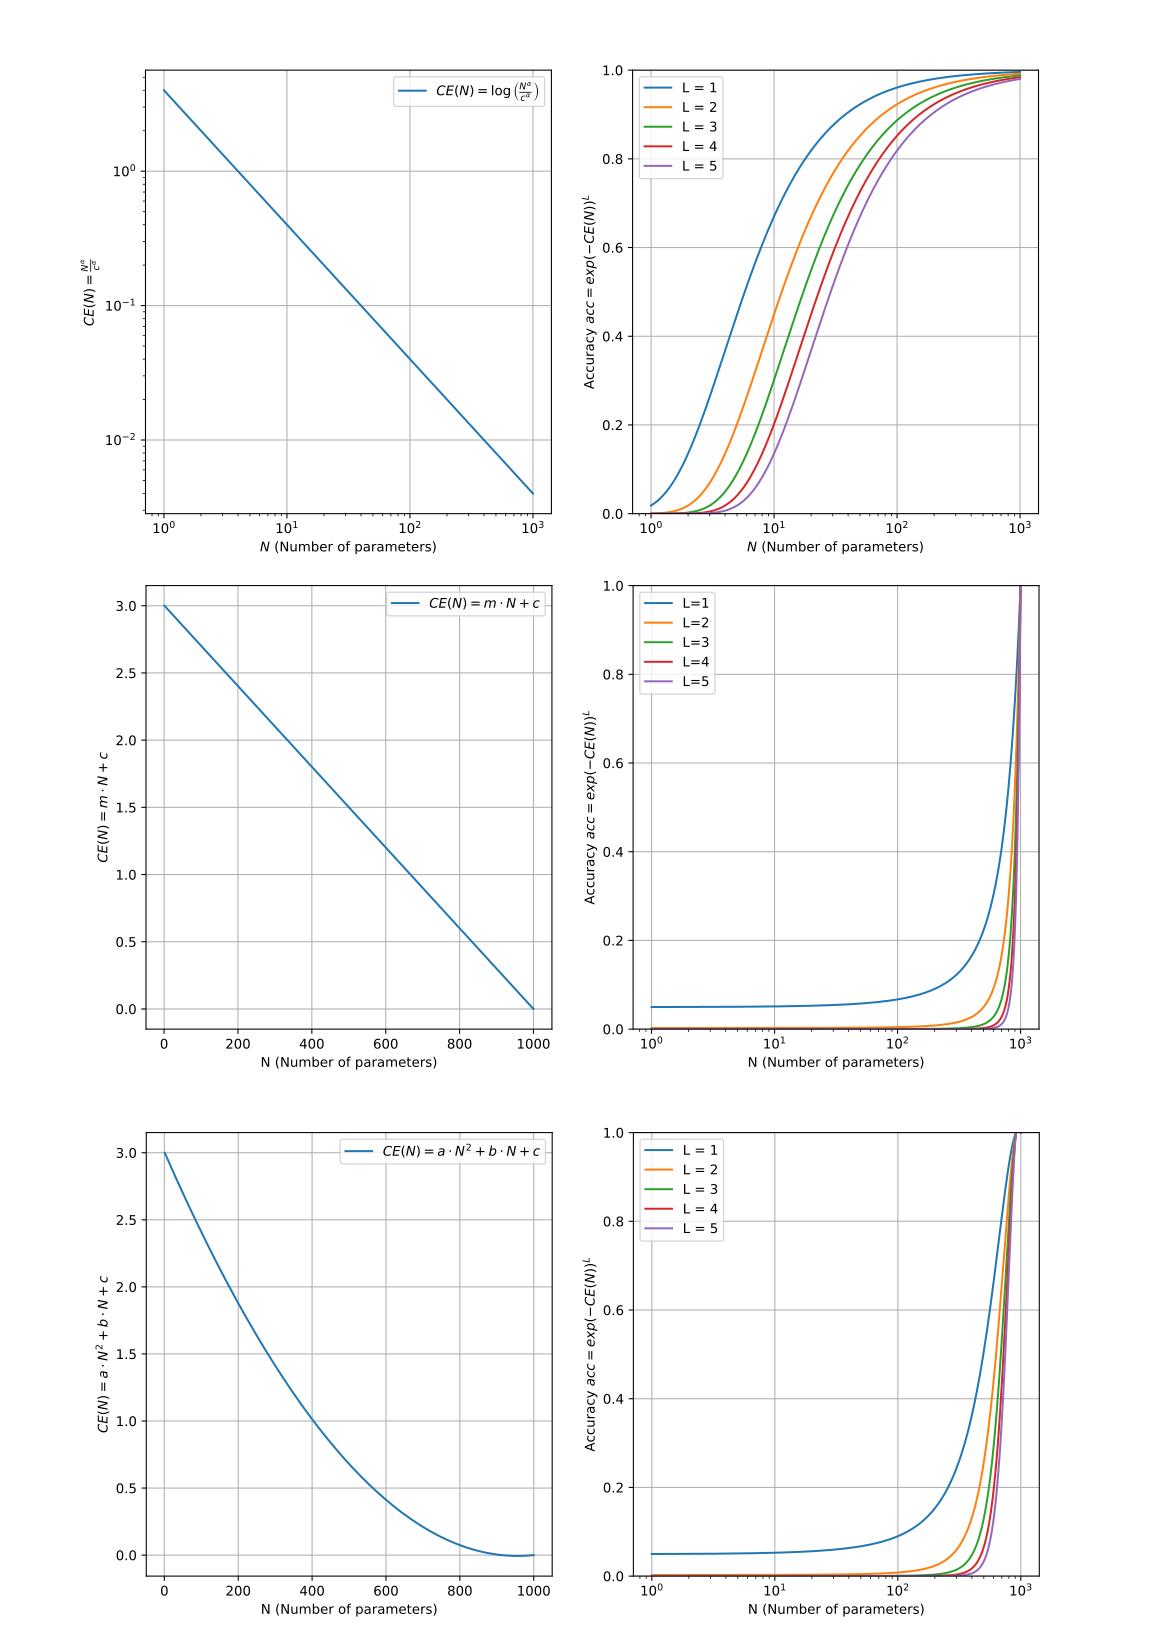
\includegraphics[width=0.8\textwidth]{figures/loss_decreasing_leads_to_emergence/decreasing_loss_leads_to_emergence_as_L_increases.png}
%   \caption{
%   \textbf{Emergence does not depend on scaling laws: any decreasing cross-entropy loss induces apparent emergence as L increases as you require more tokens to be exactly correct, i.e. L increases.}
%   The first row shows the same argument as in the main section, where a decreasing cross-entropy loss as a scaling law induces emergence as $L$ increases.
%   The second row shows the that apparent emergence is induced even when the cross-entropy loss decreases linearly.
%   The third row shows that the apparent emergence is induced when the cross-entropy loss decreases quadratically.
%   Emergence is amplified in this case especially by the increase in sharpness as more tokens are required to be correct. 
%   This means that simply changing the evaluation metric can suddenly induce emergence, and it is not an intrinsic property of the model. 
%   }
%   \label{fig:decreasing_loss_leads_to_emergence_as_L_increases}
% \end{figure}


\section{Inducing Emergent Abilities in Networks on Vision Tasks}
\label{app:sec:inducing_emergence_vision}

\subsection{Emergent Classification of MNIST Handwritten Digits by Convolutional Networks}

\begin{figure}
    \centering
    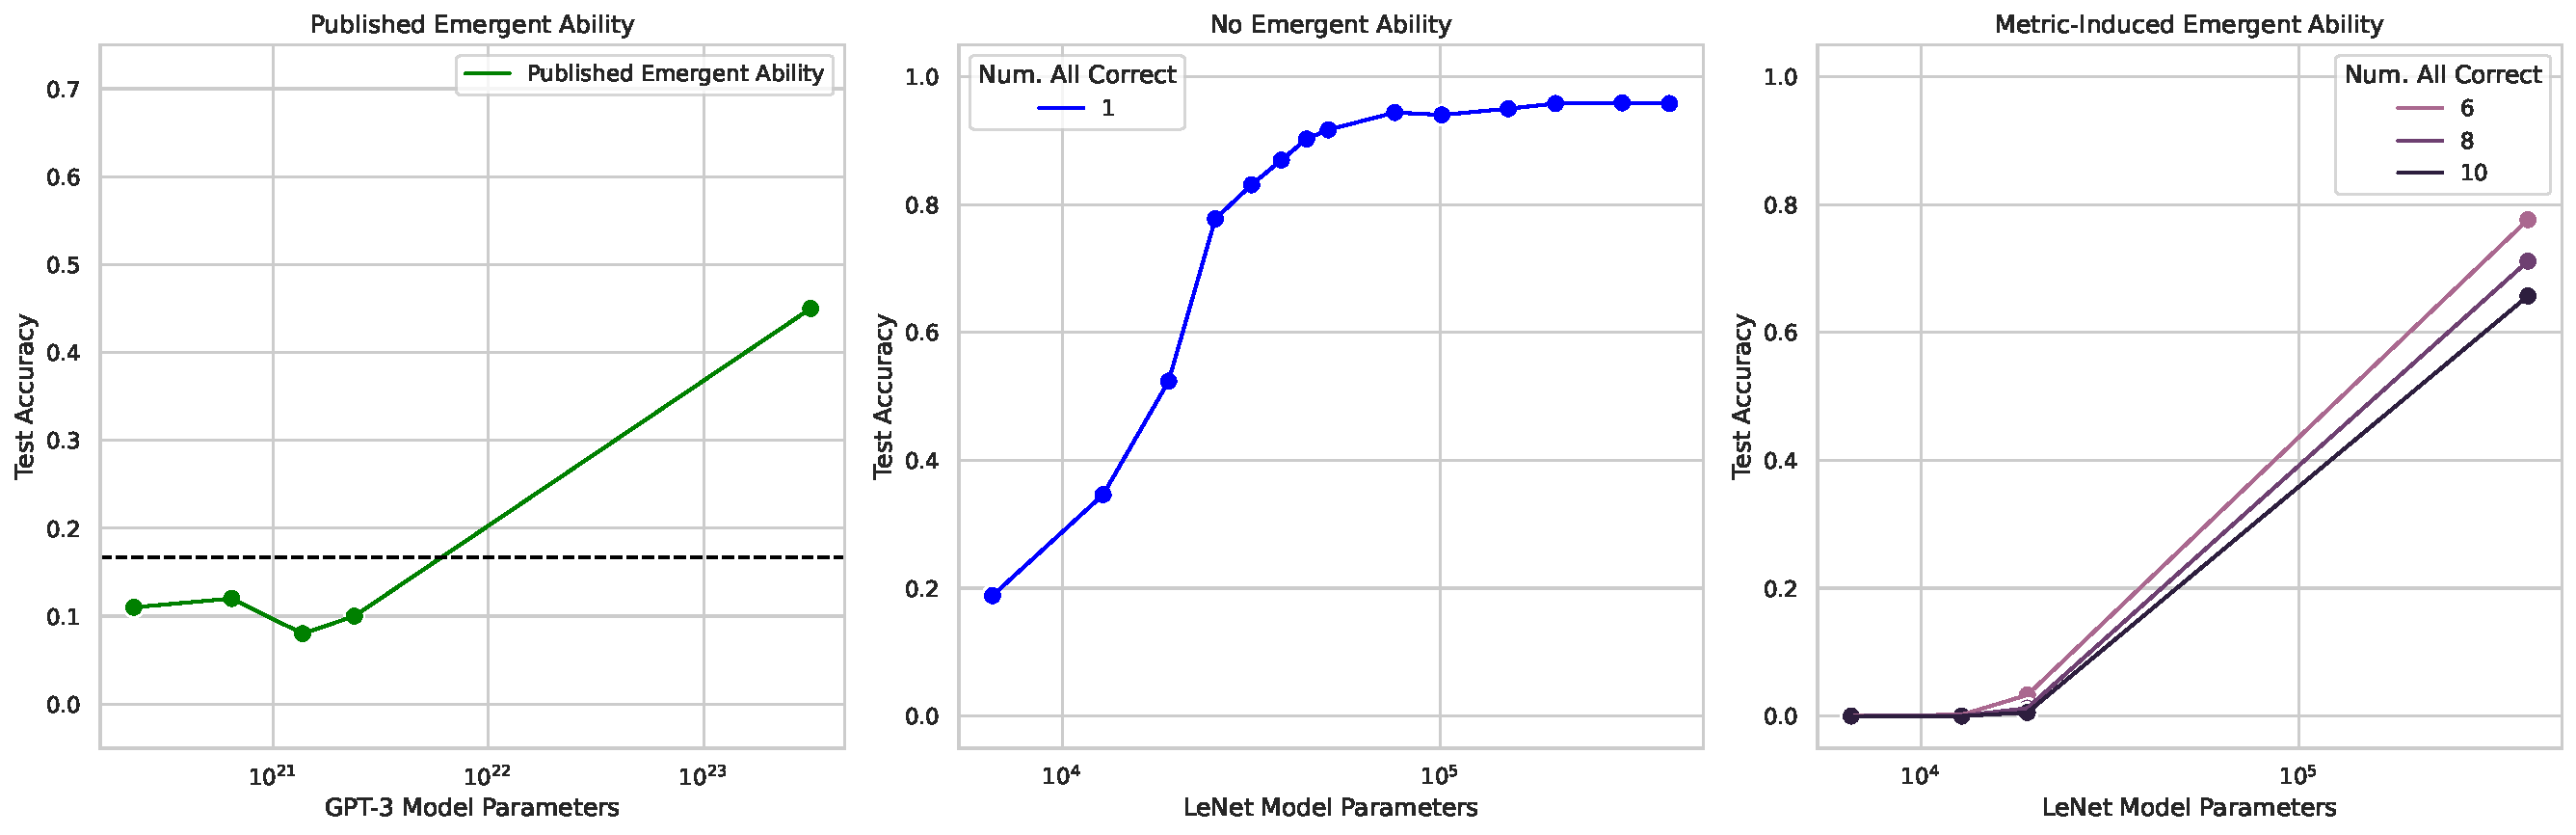
\includegraphics[width=\textwidth]{figures/vision/no_emergence_and_emergence_dataset=mnist.pdf}
    \caption{\textbf{Induced emergent MNIST classification ability in convolutional networks.} (A) A published emergent ability from the BIG-Bench Grounded Mappings task \cite{wei2022emergent}. (B) LeNet trained on MNIST \cite{lecun1998mnist} displays a predictable, commonplace sigmoidal increase in test accuracy as model parameters increase. (C) When accuracy is redefined as correctly classifying $K$ out of $K$ independent test data, this newly defined metric induces a seemingly unpredictable change.}
    \label{fig:vision_mnist}
\end{figure}

We begin by inducing an emergent classification ability in a LeNet convolutional neural network family \cite{lecun1998gradient}, trained on the MNIST handwritten digits dataset \cite{lecun1998mnist}.
This family displays smoothly increasing test accuracy as the number of parameters increase (Fig. \ref{fig:vision_mnist}B).
To emulate the accuracy metric used by emergence papers \cite{ganguli2022predictability, wei2022emergent, srivastava2022beyond}, we use \textit{subset accuracy}: 1 if the network classifies $K$ out of $K$ (independent) test data correctly, 0 otherwise.
Under this definition of accuracy, the model family displays an ``emergent" ability to correctly classify sets of MNIST digits as $K$ increases from $1$ to $5$, especially when combined with sparse sampling of model sizes (Fig. \ref{fig:vision_mnist}C).
This convolutional family's emergent classification ability qualitatively matches published emergent abilities, e.g., at the BIG-Bench Grounded Mappings task \cite{wei2022emergent} (Fig. \ref{fig:vision_mnist}A).


\end{document}